\documentclass[10pt,journal,compsoc]{IEEEtran}

\usepackage[T1]{fontenc}
\usepackage{graphicx}
\usepackage{booktabs}
\usepackage{amsmath}
\usepackage{textcomp}
\usepackage{url}
\usepackage[hidelinks]{hyperref}
\usepackage{cite}

\graphicspath{{figures/}}
% generated by make_tex.py from out/numbers_v2.json -- do not edit
\newcommand{\LatMeanA}{19.37}
\newcommand{\LatMeansdA}{0.14}
\newcommand{\LatMeanB}{20.68}
\newcommand{\LatMeansdB}{0.41}
\newcommand{\LatMeanC}{29.26}
\newcommand{\LatMeansdC}{0.82}
\newcommand{\LatMeanBA}{+1.30}
\newcommand{\LatMeanBAabs}{1.30}
\newcommand{\LatMeanBAlo}{0.52}
\newcommand{\LatMeanBAhi}{2.08}
\newcommand{\LatMeanBApct}{+6.7}
\newcommand{\LatMeanBApctabs}{6.7}
\newcommand{\LatMeanBApctlo}{2.7}
\newcommand{\LatMeanBApcthi}{10.8}
\newcommand{\LatMeanBAblkOne}{+1.64}
\newcommand{\LatMeanBAblkOneabs}{1.64}
\newcommand{\LatMeanBAblkTwo}{+1.26}
\newcommand{\LatMeanBAblkTwoabs}{1.26}
\newcommand{\LatMeanBAblkThree}{+1.01}
\newcommand{\LatMeanBAblkThreeabs}{1.01}
\newcommand{\LatMeanBAblkmin}{1.01}
\newcommand{\LatMeanBAblkmax}{1.64}
\newcommand{\LatMeanCB}{+8.58}
\newcommand{\LatMeanCBabs}{8.58}
\newcommand{\LatMeanCBlo}{5.81}
\newcommand{\LatMeanCBhi}{11.35}
\newcommand{\LatMeanCBpct}{+41.5}
\newcommand{\LatMeanCBpctabs}{41.5}
\newcommand{\LatMeanCBpctlo}{28.1}
\newcommand{\LatMeanCBpcthi}{54.9}
\newcommand{\LatMeanCBblkOne}{+7.45}
\newcommand{\LatMeanCBblkOneabs}{7.45}
\newcommand{\LatMeanCBblkTwo}{+9.68}
\newcommand{\LatMeanCBblkTwoabs}{9.68}
\newcommand{\LatMeanCBblkThree}{+8.62}
\newcommand{\LatMeanCBblkThreeabs}{8.62}
\newcommand{\LatMeanCBblkmin}{7.45}
\newcommand{\LatMeanCBblkmax}{9.68}
\newcommand{\LatMeanCA}{+9.89}
\newcommand{\LatMeanCAabs}{9.89}
\newcommand{\LatMeanCAlo}{7.52}
\newcommand{\LatMeanCAhi}{12.25}
\newcommand{\LatMeanCApct}{+51.0}
\newcommand{\LatMeanCApctabs}{51.0}
\newcommand{\LatMeanCApctlo}{38.8}
\newcommand{\LatMeanCApcthi}{63.2}
\newcommand{\LatMeanCAblkOne}{+9.09}
\newcommand{\LatMeanCAblkOneabs}{9.09}
\newcommand{\LatMeanCAblkTwo}{+10.94}
\newcommand{\LatMeanCAblkTwoabs}{10.94}
\newcommand{\LatMeanCAblkThree}{+9.63}
\newcommand{\LatMeanCAblkThreeabs}{9.63}
\newcommand{\LatMeanCAblkmin}{9.09}
\newcommand{\LatMeanCAblkmax}{10.94}
\newcommand{\LatMedA}{20.20}
\newcommand{\LatMedsdA}{0.17}
\newcommand{\LatMedB}{20.83}
\newcommand{\LatMedsdB}{1.44}
\newcommand{\LatMedC}{27.10}
\newcommand{\LatMedsdC}{2.31}
\newcommand{\LatMedBA}{+0.63}
\newcommand{\LatMedBAabs}{0.63}
\newcommand{\LatMedBAlo}{\textminus 2.76}
\newcommand{\LatMedBAhi}{4.02}
\newcommand{\LatMedBApct}{+3.1}
\newcommand{\LatMedBApctabs}{3.1}
\newcommand{\LatMedBApctlo}{\textminus 13.7}
\newcommand{\LatMedBApcthi}{19.9}
\newcommand{\LatMedBAblkOne}{+2.20}
\newcommand{\LatMedBAblkOneabs}{2.20}
\newcommand{\LatMedBAblkTwo}{+0.00}
\newcommand{\LatMedBAblkTwoabs}{0.00}
\newcommand{\LatMedBAblkThree}{\textminus 0.30}
\newcommand{\LatMedBAblkThreeabs}{0.30}
\newcommand{\LatMedBAblkmin}{0.00}
\newcommand{\LatMedBAblkmax}{2.20}
\newcommand{\LatMedCB}{+6.27}
\newcommand{\LatMedCBabs}{6.27}
\newcommand{\LatMedCBlo}{\textminus 2.30}
\newcommand{\LatMedCBhi}{14.84}
\newcommand{\LatMedCBpct}{+30.1}
\newcommand{\LatMedCBpctabs}{30.1}
\newcommand{\LatMedCBpctlo}{\textminus 11.1}
\newcommand{\LatMedCBpcthi}{71.2}
\newcommand{\LatMedCBblkOne}{+2.80}
\newcommand{\LatMedCBblkOneabs}{2.80}
\newcommand{\LatMedCBblkTwo}{+9.70}
\newcommand{\LatMedCBblkTwoabs}{9.70}
\newcommand{\LatMedCBblkThree}{+6.30}
\newcommand{\LatMedCBblkThreeabs}{6.30}
\newcommand{\LatMedCBblkmin}{2.80}
\newcommand{\LatMedCBblkmax}{9.70}
\newcommand{\LatMedCA}{+6.90}
\newcommand{\LatMedCAabs}{6.90}
\newcommand{\LatMedCAlo}{0.75}
\newcommand{\LatMedCAhi}{13.05}
\newcommand{\LatMedCApct}{+34.2}
\newcommand{\LatMedCApctabs}{34.2}
\newcommand{\LatMedCApctlo}{3.7}
\newcommand{\LatMedCApcthi}{64.6}
\newcommand{\LatMedCAblkOne}{+5.00}
\newcommand{\LatMedCAblkOneabs}{5.00}
\newcommand{\LatMedCAblkTwo}{+9.70}
\newcommand{\LatMedCAblkTwoabs}{9.70}
\newcommand{\LatMedCAblkThree}{+6.00}
\newcommand{\LatMedCAblkThreeabs}{6.00}
\newcommand{\LatMedCAblkmin}{5.00}
\newcommand{\LatMedCAblkmax}{9.70}
\newcommand{\LatPninetyfiveA}{26.00}
\newcommand{\LatPninetyfivesdA}{0.61}
\newcommand{\LatPninetyfiveB}{26.20}
\newcommand{\LatPninetyfivesdB}{1.04}
\newcommand{\LatPninetyfiveC}{41.57}
\newcommand{\LatPninetyfivesdC}{1.96}
\newcommand{\LatPninetyfiveBA}{+0.20}
\newcommand{\LatPninetyfiveBAabs}{0.20}
\newcommand{\LatPninetyfiveBAlo}{\textminus 3.30}
\newcommand{\LatPninetyfiveBAhi}{3.70}
\newcommand{\LatPninetyfiveBApct}{+0.8}
\newcommand{\LatPninetyfiveBApctabs}{0.8}
\newcommand{\LatPninetyfiveBApctlo}{\textminus 12.7}
\newcommand{\LatPninetyfiveBApcthi}{14.2}
\newcommand{\LatPninetyfiveBAblkOne}{\textminus 1.30}
\newcommand{\LatPninetyfiveBAblkOneabs}{1.30}
\newcommand{\LatPninetyfiveBAblkTwo}{+0.40}
\newcommand{\LatPninetyfiveBAblkTwoabs}{0.40}
\newcommand{\LatPninetyfiveBAblkThree}{+1.50}
\newcommand{\LatPninetyfiveBAblkThreeabs}{1.50}
\newcommand{\LatPninetyfiveBAblkmin}{0.40}
\newcommand{\LatPninetyfiveBAblkmax}{1.50}
\newcommand{\LatPninetyfiveCB}{+15.37}
\newcommand{\LatPninetyfiveCBabs}{15.37}
\newcommand{\LatPninetyfiveCBlo}{8.10}
\newcommand{\LatPninetyfiveCBhi}{22.64}
\newcommand{\LatPninetyfiveCBpct}{+58.7}
\newcommand{\LatPninetyfiveCBpctabs}{58.7}
\newcommand{\LatPninetyfiveCBpctlo}{30.9}
\newcommand{\LatPninetyfiveCBpcthi}{86.4}
\newcommand{\LatPninetyfiveCBblkOne}{+18.60}
\newcommand{\LatPninetyfiveCBblkOneabs}{18.60}
\newcommand{\LatPninetyfiveCBblkTwo}{+14.60}
\newcommand{\LatPninetyfiveCBblkTwoabs}{14.60}
\newcommand{\LatPninetyfiveCBblkThree}{+12.90}
\newcommand{\LatPninetyfiveCBblkThreeabs}{12.90}
\newcommand{\LatPninetyfiveCBblkmin}{12.90}
\newcommand{\LatPninetyfiveCBblkmax}{18.60}
\newcommand{\LatPninetyfiveCA}{+15.57}
\newcommand{\LatPninetyfiveCAabs}{15.57}
\newcommand{\LatPninetyfiveCAlo}{11.76}
\newcommand{\LatPninetyfiveCAhi}{19.37}
\newcommand{\LatPninetyfiveCApct}{+59.9}
\newcommand{\LatPninetyfiveCApctabs}{59.9}
\newcommand{\LatPninetyfiveCApctlo}{45.2}
\newcommand{\LatPninetyfiveCApcthi}{74.5}
\newcommand{\LatPninetyfiveCAblkOne}{+17.30}
\newcommand{\LatPninetyfiveCAblkOneabs}{17.30}
\newcommand{\LatPninetyfiveCAblkTwo}{+15.00}
\newcommand{\LatPninetyfiveCAblkTwoabs}{15.00}
\newcommand{\LatPninetyfiveCAblkThree}{+14.40}
\newcommand{\LatPninetyfiveCAblkThreeabs}{14.40}
\newcommand{\LatPninetyfiveCAblkmin}{14.40}
\newcommand{\LatPninetyfiveCAblkmax}{17.30}
\newcommand{\LatPninetynineA}{28.90}
\newcommand{\LatPninetyninesdA}{0.80}
\newcommand{\LatPninetynineB}{31.45}
\newcommand{\LatPninetyninesdB}{1.51}
\newcommand{\LatPninetynineC}{43.83}
\newcommand{\LatPninetyninesdC}{0.15}
\newcommand{\LatPninetynineBA}{+2.55}
\newcommand{\LatPninetynineBAabs}{2.55}
\newcommand{\LatPninetynineBAlo}{\textminus 1.79}
\newcommand{\LatPninetynineBAhi}{6.90}
\newcommand{\LatPninetynineBApct}{+8.8}
\newcommand{\LatPninetynineBApctabs}{8.8}
\newcommand{\LatPninetynineBApctlo}{\textminus 6.2}
\newcommand{\LatPninetynineBApcthi}{23.9}
\newcommand{\LatPninetynineBAblkOne}{+4.30}
\newcommand{\LatPninetynineBAblkOneabs}{4.30}
\newcommand{\LatPninetynineBAblkTwo}{+0.80}
\newcommand{\LatPninetynineBAblkTwoabs}{0.80}
\newcommand{\LatPninetynineBAblkThree}{+2.56}
\newcommand{\LatPninetynineBAblkThreeabs}{2.56}
\newcommand{\LatPninetynineBAblkmin}{0.80}
\newcommand{\LatPninetynineBAblkmax}{4.30}
\newcommand{\LatPninetynineCB}{+12.38}
\newcommand{\LatPninetynineCBabs}{12.38}
\newcommand{\LatPninetynineCBlo}{8.98}
\newcommand{\LatPninetynineCBhi}{15.78}
\newcommand{\LatPninetynineCBpct}{+39.4}
\newcommand{\LatPninetynineCBpctabs}{39.4}
\newcommand{\LatPninetynineCBpctlo}{28.6}
\newcommand{\LatPninetynineCBpcthi}{50.2}
\newcommand{\LatPninetynineCBblkOne}{+10.80}
\newcommand{\LatPninetynineCBblkOneabs}{10.80}
\newcommand{\LatPninetynineCBblkTwo}{+13.20}
\newcommand{\LatPninetynineCBblkTwoabs}{13.20}
\newcommand{\LatPninetynineCBblkThree}{+13.14}
\newcommand{\LatPninetynineCBblkThreeabs}{13.14}
\newcommand{\LatPninetynineCBblkmin}{10.80}
\newcommand{\LatPninetynineCBblkmax}{13.20}
\newcommand{\LatPninetynineCA}{+14.93}
\newcommand{\LatPninetynineCAabs}{14.93}
\newcommand{\LatPninetynineCAlo}{12.79}
\newcommand{\LatPninetynineCAhi}{17.08}
\newcommand{\LatPninetynineCApct}{+51.7}
\newcommand{\LatPninetynineCApctabs}{51.7}
\newcommand{\LatPninetynineCApctlo}{44.3}
\newcommand{\LatPninetynineCApcthi}{59.1}
\newcommand{\LatPninetynineCAblkOne}{+15.10}
\newcommand{\LatPninetynineCAblkOneabs}{15.10}
\newcommand{\LatPninetynineCAblkTwo}{+14.00}
\newcommand{\LatPninetynineCAblkTwoabs}{14.00}
\newcommand{\LatPninetynineCAblkThree}{+15.70}
\newcommand{\LatPninetynineCAblkThreeabs}{15.70}
\newcommand{\LatPninetynineCAblkmin}{14.00}
\newcommand{\LatPninetynineCAblkmax}{15.70}
\newcommand{\LatSDA}{3.88}
\newcommand{\LatSDsdA}{0.12}
\newcommand{\LatSDB}{4.11}
\newcommand{\LatSDsdB}{0.12}
\newcommand{\LatSDC}{5.08}
\newcommand{\LatSDsdC}{0.31}
\newcommand{\LatSDBA}{+0.23}
\newcommand{\LatSDBAabs}{0.23}
\newcommand{\LatSDBAlo}{\textminus 0.20}
\newcommand{\LatSDBAhi}{0.66}
\newcommand{\LatSDBApct}{+5.9}
\newcommand{\LatSDBApctabs}{5.9}
\newcommand{\LatSDBApctlo}{\textminus 5.2}
\newcommand{\LatSDBApcthi}{17.1}
\newcommand{\LatSDBAblkOne}{+0.12}
\newcommand{\LatSDBAblkOneabs}{0.12}
\newcommand{\LatSDBAblkTwo}{+0.14}
\newcommand{\LatSDBAblkTwoabs}{0.14}
\newcommand{\LatSDBAblkThree}{+0.43}
\newcommand{\LatSDBAblkThreeabs}{0.43}
\newcommand{\LatSDBAblkmin}{0.12}
\newcommand{\LatSDBAblkmax}{0.43}
\newcommand{\LatSDCB}{+0.97}
\newcommand{\LatSDCBabs}{0.97}
\newcommand{\LatSDCBlo}{\textminus 0.11}
\newcommand{\LatSDCBhi}{2.05}
\newcommand{\LatSDCBpct}{+23.6}
\newcommand{\LatSDCBpctabs}{23.6}
\newcommand{\LatSDCBpctlo}{\textminus 2.6}
\newcommand{\LatSDCBpcthi}{49.8}
\newcommand{\LatSDCBblkOne}{+1.47}
\newcommand{\LatSDCBblkOneabs}{1.47}
\newcommand{\LatSDCBblkTwo}{+0.74}
\newcommand{\LatSDCBblkTwoabs}{0.74}
\newcommand{\LatSDCBblkThree}{+0.69}
\newcommand{\LatSDCBblkThreeabs}{0.69}
\newcommand{\LatSDCBblkmin}{0.69}
\newcommand{\LatSDCBblkmax}{1.47}
\newcommand{\LatSDCA}{+1.20}
\newcommand{\LatSDCAabs}{1.20}
\newcommand{\LatSDCAlo}{0.31}
\newcommand{\LatSDCAhi}{2.08}
\newcommand{\LatSDCApct}{+30.9}
\newcommand{\LatSDCApctabs}{30.9}
\newcommand{\LatSDCApctlo}{8.1}
\newcommand{\LatSDCApcthi}{53.7}
\newcommand{\LatSDCAblkOne}{+1.59}
\newcommand{\LatSDCAblkOneabs}{1.59}
\newcommand{\LatSDCAblkTwo}{+0.89}
\newcommand{\LatSDCAblkTwoabs}{0.89}
\newcommand{\LatSDCAblkThree}{+1.12}
\newcommand{\LatSDCAblkThreeabs}{1.12}
\newcommand{\LatSDCAblkmin}{0.89}
\newcommand{\LatSDCAblkmax}{1.59}
\newcommand{\LatPoneA}{14.9}
\newcommand{\LatPonesdA}{0.2}
\newcommand{\LatPoneB}{14.7}
\newcommand{\LatPonesdB}{0.1}
\newcommand{\LatPoneC}{24.6}
\newcommand{\LatPonesdC}{0.1}
\newcommand{\LatPoneBA}{\textminus 0.2}
\newcommand{\LatPoneBAabs}{0.2}
\newcommand{\LatPoneBAlo}{\textminus 0.5}
\newcommand{\LatPoneBAhi}{0.2}
\newcommand{\LatPoneBApct}{\textminus 1.1}
\newcommand{\LatPoneBApctabs}{1.1}
\newcommand{\LatPoneBApctlo}{\textminus 3.7}
\newcommand{\LatPoneBApcthi}{1.4}
\newcommand{\LatPoneBAblkOne}{\textminus 0.2}
\newcommand{\LatPoneBAblkOneabs}{0.2}
\newcommand{\LatPoneBAblkTwo}{+0.0}
\newcommand{\LatPoneBAblkTwoabs}{0.0}
\newcommand{\LatPoneBAblkThree}{\textminus 0.3}
\newcommand{\LatPoneBAblkThreeabs}{0.3}
\newcommand{\LatPoneBAblkmin}{0.0}
\newcommand{\LatPoneBAblkmax}{\textminus 0.3}
\newcommand{\LatPoneCB}{+9.8}
\newcommand{\LatPoneCBabs}{9.8}
\newcommand{\LatPoneCBlo}{9.7}
\newcommand{\LatPoneCBhi}{10.0}
\newcommand{\LatPoneCBpct}{+66.7}
\newcommand{\LatPoneCBpctabs}{66.7}
\newcommand{\LatPoneCBpctlo}{65.8}
\newcommand{\LatPoneCBpcthi}{67.7}
\newcommand{\LatPoneCBblkOne}{+9.8}
\newcommand{\LatPoneCBblkOneabs}{9.8}
\newcommand{\LatPoneCBblkTwo}{+9.8}
\newcommand{\LatPoneCBblkTwoabs}{9.8}
\newcommand{\LatPoneCBblkThree}{+9.9}
\newcommand{\LatPoneCBblkThreeabs}{9.9}
\newcommand{\LatPoneCBblkmin}{9.8}
\newcommand{\LatPoneCBblkmax}{9.9}
\newcommand{\LatPoneCA}{+9.7}
\newcommand{\LatPoneCAabs}{9.7}
\newcommand{\LatPoneCAlo}{9.4}
\newcommand{\LatPoneCAhi}{10.0}
\newcommand{\LatPoneCApct}{+64.9}
\newcommand{\LatPoneCApctabs}{64.9}
\newcommand{\LatPoneCApctlo}{63.0}
\newcommand{\LatPoneCApcthi}{66.8}
\newcommand{\LatPoneCAblkOne}{+9.6}
\newcommand{\LatPoneCAblkOneabs}{9.6}
\newcommand{\LatPoneCAblkTwo}{+9.8}
\newcommand{\LatPoneCAblkTwoabs}{9.8}
\newcommand{\LatPoneCAblkThree}{+9.6}
\newcommand{\LatPoneCAblkThreeabs}{9.6}
\newcommand{\LatPoneCAblkmin}{9.6}
\newcommand{\LatPoneCAblkmax}{9.8}
\newcommand{\FastA}{42}
\newcommand{\FastsdA}{1}
\newcommand{\FastB}{24}
\newcommand{\FastsdB}{4}
\newcommand{\FastC}{0}
\newcommand{\FastsdC}{0}
\newcommand{\FastBA}{\textminus 18}
\newcommand{\FastBAabs}{18}
\newcommand{\FastBAlo}{\textminus 25}
\newcommand{\FastBAhi}{\textminus 12}
\newcommand{\FastBApct}{\textminus 43.6}
\newcommand{\FastBApctabs}{43.6}
\newcommand{\FastBApctlo}{\textminus 59.1}
\newcommand{\FastBApcthi}{\textminus 28.0}
\newcommand{\FastBAblkOne}{\textminus 21}
\newcommand{\FastBAblkOneabs}{21}
\newcommand{\FastBAblkTwo}{\textminus 17}
\newcommand{\FastBAblkTwoabs}{17}
\newcommand{\FastBAblkThree}{\textminus 16}
\newcommand{\FastBAblkThreeabs}{16}
\newcommand{\FastBAblkmin}{\textminus 16}
\newcommand{\FastBAblkmax}{\textminus 21}
\newcommand{\FastCB}{\textminus 24}
\newcommand{\FastCBabs}{24}
\newcommand{\FastCBlo}{\textminus 33}
\newcommand{\FastCBhi}{\textminus 14}
\newcommand{\FastCBpct}{\textminus 100.0}
\newcommand{\FastCBpctabs}{100.0}
\newcommand{\FastCBpctlo}{\textminus 138.5}
\newcommand{\FastCBpcthi}{\textminus 61.5}
\newcommand{\FastCBblkOne}{\textminus 19}
\newcommand{\FastCBblkOneabs}{19}
\newcommand{\FastCBblkTwo}{\textminus 25}
\newcommand{\FastCBblkTwoabs}{25}
\newcommand{\FastCBblkThree}{\textminus 26}
\newcommand{\FastCBblkThreeabs}{26}
\newcommand{\FastCBblkmin}{\textminus 19}
\newcommand{\FastCBblkmax}{\textminus 26}
\newcommand{\FastCA}{\textminus 42}
\newcommand{\FastCAabs}{42}
\newcommand{\FastCAlo}{\textminus 45}
\newcommand{\FastCAhi}{\textminus 39}
\newcommand{\FastCApct}{\textminus 100.0}
\newcommand{\FastCApctabs}{100.0}
\newcommand{\FastCApctlo}{\textminus 107.0}
\newcommand{\FastCApcthi}{\textminus 93.0}
\newcommand{\FastCAblkOne}{\textminus 40}
\newcommand{\FastCAblkOneabs}{40}
\newcommand{\FastCAblkTwo}{\textminus 43}
\newcommand{\FastCAblkTwoabs}{43}
\newcommand{\FastCAblkThree}{\textminus 42}
\newcommand{\FastCAblkThreeabs}{42}
\newcommand{\FastCAblkmin}{\textminus 40}
\newcommand{\FastCAblkmax}{\textminus 43}
\newcommand{\CPUA}{56.1}
\newcommand{\CPUsdA}{0.2}
\newcommand{\CPUB}{57.3}
\newcommand{\CPUsdB}{0.7}
\newcommand{\CPUC}{48.6}
\newcommand{\CPUsdC}{0.4}
\newcommand{\CPUBA}{+1.3}
\newcommand{\CPUBAabs}{1.3}
\newcommand{\CPUBAlo}{\textminus 0.1}
\newcommand{\CPUBAhi}{2.6}
\newcommand{\CPUBApct}{+2.2}
\newcommand{\CPUBApctabs}{2.2}
\newcommand{\CPUBApctlo}{\textminus 0.2}
\newcommand{\CPUBApcthi}{4.7}
\newcommand{\CPUBAblkOne}{+1.9}
\newcommand{\CPUBAblkOneabs}{1.9}
\newcommand{\CPUBAblkTwo}{+1.1}
\newcommand{\CPUBAblkTwoabs}{1.1}
\newcommand{\CPUBAblkThree}{+0.8}
\newcommand{\CPUBAblkThreeabs}{0.8}
\newcommand{\CPUBAblkmin}{0.8}
\newcommand{\CPUBAblkmax}{1.9}
\newcommand{\CPUCB}{\textminus 8.8}
\newcommand{\CPUCBabs}{8.8}
\newcommand{\CPUCBlo}{\textminus 10.8}
\newcommand{\CPUCBhi}{\textminus 6.8}
\newcommand{\CPUCBpct}{\textminus 15.3}
\newcommand{\CPUCBpctabs}{15.3}
\newcommand{\CPUCBpctlo}{\textminus 18.8}
\newcommand{\CPUCBpcthi}{\textminus 11.8}
\newcommand{\CPUCBblkOne}{\textminus 9.6}
\newcommand{\CPUCBblkOneabs}{9.6}
\newcommand{\CPUCBblkTwo}{\textminus 8.0}
\newcommand{\CPUCBblkTwoabs}{8.0}
\newcommand{\CPUCBblkThree}{\textminus 8.7}
\newcommand{\CPUCBblkThreeabs}{8.7}
\newcommand{\CPUCBblkmin}{\textminus 8.0}
\newcommand{\CPUCBblkmax}{\textminus 9.6}
\newcommand{\CPUCA}{\textminus 7.5}
\newcommand{\CPUCAabs}{7.5}
\newcommand{\CPUCAlo}{\textminus 8.8}
\newcommand{\CPUCAhi}{\textminus 6.2}
\newcommand{\CPUCApct}{\textminus 13.4}
\newcommand{\CPUCApctabs}{13.4}
\newcommand{\CPUCApctlo}{\textminus 15.7}
\newcommand{\CPUCApcthi}{\textminus 11.0}
\newcommand{\CPUCAblkOne}{\textminus 7.7}
\newcommand{\CPUCAblkOneabs}{7.7}
\newcommand{\CPUCAblkTwo}{\textminus 6.9}
\newcommand{\CPUCAblkTwoabs}{6.9}
\newcommand{\CPUCAblkThree}{\textminus 7.9}
\newcommand{\CPUCAblkThreeabs}{7.9}
\newcommand{\CPUCAblkmin}{\textminus 6.9}
\newcommand{\CPUCAblkmax}{\textminus 7.9}
\newcommand{\CPUmsA}{150.6}
\newcommand{\CPUmssdA}{0.4}
\newcommand{\CPUmsB}{153.4}
\newcommand{\CPUmssdB}{0.9}
\newcommand{\CPUmsC}{130.0}
\newcommand{\CPUmssdC}{1.4}
\newcommand{\CPUmsBA}{+2.8}
\newcommand{\CPUmsBAabs}{2.8}
\newcommand{\CPUmsBAlo}{0.9}
\newcommand{\CPUmsBAhi}{4.8}
\newcommand{\CPUmsBApct}{+1.9}
\newcommand{\CPUmsBApctabs}{1.9}
\newcommand{\CPUmsBApctlo}{0.6}
\newcommand{\CPUmsBApcthi}{3.2}
\newcommand{\CPUmsBAblkOne}{+3.6}
\newcommand{\CPUmsBAblkOneabs}{3.6}
\newcommand{\CPUmsBAblkTwo}{+2.9}
\newcommand{\CPUmsBAblkTwoabs}{2.9}
\newcommand{\CPUmsBAblkThree}{+2.0}
\newcommand{\CPUmsBAblkThreeabs}{2.0}
\newcommand{\CPUmsBAblkmin}{2.0}
\newcommand{\CPUmsBAblkmax}{3.6}
\newcommand{\CPUmsCB}{\textminus 23.4}
\newcommand{\CPUmsCBabs}{23.4}
\newcommand{\CPUmsCBlo}{\textminus 28.4}
\newcommand{\CPUmsCBhi}{\textminus 18.3}
\newcommand{\CPUmsCBpct}{\textminus 15.2}
\newcommand{\CPUmsCBpctabs}{15.2}
\newcommand{\CPUmsCBpctlo}{\textminus 18.5}
\newcommand{\CPUmsCBpcthi}{\textminus 12.0}
\newcommand{\CPUmsCBblkOne}{\textminus 25.4}
\newcommand{\CPUmsCBblkOneabs}{25.4}
\newcommand{\CPUmsCBblkTwo}{\textminus 21.4}
\newcommand{\CPUmsCBblkTwoabs}{21.4}
\newcommand{\CPUmsCBblkThree}{\textminus 23.3}
\newcommand{\CPUmsCBblkThreeabs}{23.3}
\newcommand{\CPUmsCBblkmin}{\textminus 21.4}
\newcommand{\CPUmsCBblkmax}{\textminus 25.4}
\newcommand{\CPUmsCA}{\textminus 20.5}
\newcommand{\CPUmsCAabs}{20.5}
\newcommand{\CPUmsCAlo}{\textminus 25.0}
\newcommand{\CPUmsCAhi}{\textminus 16.1}
\newcommand{\CPUmsCApct}{\textminus 13.6}
\newcommand{\CPUmsCApctabs}{13.6}
\newcommand{\CPUmsCApctlo}{\textminus 16.6}
\newcommand{\CPUmsCApcthi}{\textminus 10.7}
\newcommand{\CPUmsCAblkOne}{\textminus 21.8}
\newcommand{\CPUmsCAblkOneabs}{21.8}
\newcommand{\CPUmsCAblkTwo}{\textminus 18.5}
\newcommand{\CPUmsCAblkTwoabs}{18.5}
\newcommand{\CPUmsCAblkThree}{\textminus 21.3}
\newcommand{\CPUmsCAblkThreeabs}{21.3}
\newcommand{\CPUmsCAblkmin}{\textminus 18.5}
\newcommand{\CPUmsCAblkmax}{\textminus 21.8}
\newcommand{\PActA}{10.46}
\newcommand{\PActsdA}{0.08}
\newcommand{\PActB}{10.51}
\newcommand{\PActsdB}{0.03}
\newcommand{\PActC}{9.81}
\newcommand{\PActsdC}{0.19}
\newcommand{\PActBA}{+0.06}
\newcommand{\PActBAabs}{0.06}
\newcommand{\PActBAlo}{\textminus 0.08}
\newcommand{\PActBAhi}{0.19}
\newcommand{\PActBApct}{+0.5}
\newcommand{\PActBApctabs}{0.5}
\newcommand{\PActBApctlo}{\textminus 0.8}
\newcommand{\PActBApcthi}{1.8}
\newcommand{\PActBAblkOne}{+0.01}
\newcommand{\PActBAblkOneabs}{0.01}
\newcommand{\PActBAblkTwo}{+0.05}
\newcommand{\PActBAblkTwoabs}{0.05}
\newcommand{\PActBAblkThree}{+0.11}
\newcommand{\PActBAblkThreeabs}{0.11}
\newcommand{\PActBAblkmin}{0.01}
\newcommand{\PActBAblkmax}{0.11}
\newcommand{\PActCB}{\textminus 0.70}
\newcommand{\PActCBabs}{0.70}
\newcommand{\PActCBlo}{\textminus 1.20}
\newcommand{\PActCBhi}{\textminus 0.20}
\newcommand{\PActCBpct}{\textminus 6.7}
\newcommand{\PActCBpctabs}{6.7}
\newcommand{\PActCBpctlo}{\textminus 11.4}
\newcommand{\PActCBpcthi}{\textminus 1.9}
\newcommand{\PActCBblkOne}{\textminus 0.84}
\newcommand{\PActCBblkOneabs}{0.84}
\newcommand{\PActCBblkTwo}{\textminus 0.47}
\newcommand{\PActCBblkTwoabs}{0.47}
\newcommand{\PActCBblkThree}{\textminus 0.79}
\newcommand{\PActCBblkThreeabs}{0.79}
\newcommand{\PActCBblkmin}{\textminus 0.47}
\newcommand{\PActCBblkmax}{\textminus 0.84}
\newcommand{\PActCA}{\textminus 0.64}
\newcommand{\PActCAabs}{0.64}
\newcommand{\PActCAlo}{\textminus 1.15}
\newcommand{\PActCAhi}{\textminus 0.13}
\newcommand{\PActCApct}{\textminus 6.2}
\newcommand{\PActCApctabs}{6.2}
\newcommand{\PActCApctlo}{\textminus 11.0}
\newcommand{\PActCApcthi}{\textminus 1.3}
\newcommand{\PActCAblkOne}{\textminus 0.83}
\newcommand{\PActCAblkOneabs}{0.83}
\newcommand{\PActCAblkTwo}{\textminus 0.42}
\newcommand{\PActCAblkTwoabs}{0.42}
\newcommand{\PActCAblkThree}{\textminus 0.68}
\newcommand{\PActCAblkThreeabs}{0.68}
\newcommand{\PActCAblkmin}{\textminus 0.42}
\newcommand{\PActCAblkmax}{\textminus 0.83}
\newcommand{\PSlpA}{6.97}
\newcommand{\PSlpsdA}{0.05}
\newcommand{\PSlpB}{6.95}
\newcommand{\PSlpsdB}{0.02}
\newcommand{\PSlpC}{6.81}
\newcommand{\PSlpsdC}{0.20}
\newcommand{\PSlpBA}{\textminus 0.02}
\newcommand{\PSlpBAabs}{0.02}
\newcommand{\PSlpBAlo}{\textminus 0.14}
\newcommand{\PSlpBAhi}{0.11}
\newcommand{\PSlpBApct}{\textminus 0.2}
\newcommand{\PSlpBApctabs}{0.2}
\newcommand{\PSlpBApctlo}{\textminus 2.0}
\newcommand{\PSlpBApcthi}{1.6}
\newcommand{\PSlpBAblkOne}{\textminus 0.05}
\newcommand{\PSlpBAblkOneabs}{0.05}
\newcommand{\PSlpBAblkTwo}{\textminus 0.04}
\newcommand{\PSlpBAblkTwoabs}{0.04}
\newcommand{\PSlpBAblkThree}{+0.04}
\newcommand{\PSlpBAblkThreeabs}{0.04}
\newcommand{\PSlpBAblkmin}{0.04}
\newcommand{\PSlpBAblkmax}{\textminus 0.05}
\newcommand{\PSlpCB}{\textminus 0.14}
\newcommand{\PSlpCBabs}{0.14}
\newcommand{\PSlpCBlo}{\textminus 0.67}
\newcommand{\PSlpCBhi}{0.39}
\newcommand{\PSlpCBpct}{\textminus 2.0}
\newcommand{\PSlpCBpctabs}{2.0}
\newcommand{\PSlpCBpctlo}{\textminus 9.6}
\newcommand{\PSlpCBpcthi}{5.7}
\newcommand{\PSlpCBblkOne}{\textminus 0.24}
\newcommand{\PSlpCBblkOneabs}{0.24}
\newcommand{\PSlpCBblkTwo}{+0.11}
\newcommand{\PSlpCBblkTwoabs}{0.11}
\newcommand{\PSlpCBblkThree}{\textminus 0.28}
\newcommand{\PSlpCBblkThreeabs}{0.28}
\newcommand{\PSlpCBblkmin}{0.11}
\newcommand{\PSlpCBblkmax}{\textminus 0.28}
\newcommand{\PSlpCA}{\textminus 0.15}
\newcommand{\PSlpCAabs}{0.15}
\newcommand{\PSlpCAlo}{\textminus 0.63}
\newcommand{\PSlpCAhi}{0.32}
\newcommand{\PSlpCApct}{\textminus 2.2}
\newcommand{\PSlpCApctabs}{2.2}
\newcommand{\PSlpCApctlo}{\textminus 9.0}
\newcommand{\PSlpCApcthi}{4.6}
\newcommand{\PSlpCAblkOne}{\textminus 0.28}
\newcommand{\PSlpCAblkOneabs}{0.28}
\newcommand{\PSlpCAblkTwo}{+0.06}
\newcommand{\PSlpCAblkTwoabs}{0.06}
\newcommand{\PSlpCAblkThree}{\textminus 0.24}
\newcommand{\PSlpCAblkThreeabs}{0.24}
\newcommand{\PSlpCAblkmin}{0.06}
\newcommand{\PSlpCAblkmax}{\textminus 0.28}
\newcommand{\PFloorA}{6.61}
\newcommand{\PFloorsdA}{0.06}
\newcommand{\PFloorB}{6.60}
\newcommand{\PFloorsdB}{0.05}
\newcommand{\PFloorC}{6.54}
\newcommand{\PFloorsdC}{0.18}
\newcommand{\PFloorBA}{\textminus 0.02}
\newcommand{\PFloorBAabs}{0.02}
\newcommand{\PFloorBAlo}{\textminus 0.11}
\newcommand{\PFloorBAhi}{0.08}
\newcommand{\PFloorBApct}{\textminus 0.3}
\newcommand{\PFloorBApctabs}{0.3}
\newcommand{\PFloorBApctlo}{\textminus 1.7}
\newcommand{\PFloorBApcthi}{1.2}
\newcommand{\PFloorBAblkOne}{\textminus 0.02}
\newcommand{\PFloorBAblkOneabs}{0.02}
\newcommand{\PFloorBAblkTwo}{\textminus 0.05}
\newcommand{\PFloorBAblkTwoabs}{0.05}
\newcommand{\PFloorBAblkThree}{+0.02}
\newcommand{\PFloorBAblkThreeabs}{0.02}
\newcommand{\PFloorBAblkmin}{\textminus 0.02}
\newcommand{\PFloorBAblkmax}{\textminus 0.05}
\newcommand{\PFloorCB}{\textminus 0.06}
\newcommand{\PFloorCBabs}{0.06}
\newcommand{\PFloorCBlo}{\textminus 0.53}
\newcommand{\PFloorCBhi}{0.41}
\newcommand{\PFloorCBpct}{\textminus 0.9}
\newcommand{\PFloorCBpctabs}{0.9}
\newcommand{\PFloorCBpctlo}{\textminus 8.1}
\newcommand{\PFloorCBpcthi}{6.2}
\newcommand{\PFloorCBblkOne}{\textminus 0.10}
\newcommand{\PFloorCBblkOneabs}{0.10}
\newcommand{\PFloorCBblkTwo}{+0.14}
\newcommand{\PFloorCBblkTwoabs}{0.14}
\newcommand{\PFloorCBblkThree}{\textminus 0.23}
\newcommand{\PFloorCBblkThreeabs}{0.23}
\newcommand{\PFloorCBblkmin}{\textminus 0.10}
\newcommand{\PFloorCBblkmax}{\textminus 0.23}
\newcommand{\PFloorCA}{\textminus 0.08}
\newcommand{\PFloorCAabs}{0.08}
\newcommand{\PFloorCAlo}{\textminus 0.46}
\newcommand{\PFloorCAhi}{0.30}
\newcommand{\PFloorCApct}{\textminus 1.2}
\newcommand{\PFloorCApctabs}{1.2}
\newcommand{\PFloorCApctlo}{\textminus 7.0}
\newcommand{\PFloorCApcthi}{4.6}
\newcommand{\PFloorCAblkOne}{\textminus 0.12}
\newcommand{\PFloorCAblkOneabs}{0.12}
\newcommand{\PFloorCAblkTwo}{+0.09}
\newcommand{\PFloorCAblkTwoabs}{0.09}
\newcommand{\PFloorCAblkThree}{\textminus 0.21}
\newcommand{\PFloorCAblkThreeabs}{0.21}
\newcommand{\PFloorCAblkmin}{0.09}
\newcommand{\PFloorCAblkmax}{\textminus 0.21}
\newcommand{\PHoldA}{7.49}
\newcommand{\PHoldsdA}{0.05}
\newcommand{\PHoldB}{7.48}
\newcommand{\PHoldsdB}{0.03}
\newcommand{\PHoldC}{7.23}
\newcommand{\PHoldsdC}{0.27}
\newcommand{\PHoldBA}{\textminus 0.01}
\newcommand{\PHoldBAabs}{0.01}
\newcommand{\PHoldBAlo}{\textminus 0.19}
\newcommand{\PHoldBAhi}{0.17}
\newcommand{\PHoldBApct}{\textminus 0.2}
\newcommand{\PHoldBApctabs}{0.2}
\newcommand{\PHoldBApctlo}{\textminus 2.6}
\newcommand{\PHoldBApcthi}{2.2}
\newcommand{\PHoldBAblkOne}{\textminus 0.08}
\newcommand{\PHoldBAblkOneabs}{0.08}
\newcommand{\PHoldBAblkTwo}{\textminus 0.03}
\newcommand{\PHoldBAblkTwoabs}{0.03}
\newcommand{\PHoldBAblkThree}{+0.07}
\newcommand{\PHoldBAblkThreeabs}{0.07}
\newcommand{\PHoldBAblkmin}{\textminus 0.03}
\newcommand{\PHoldBAblkmax}{\textminus 0.08}
\newcommand{\PHoldCB}{\textminus 0.25}
\newcommand{\PHoldCBabs}{0.25}
\newcommand{\PHoldCBlo}{\textminus 0.92}
\newcommand{\PHoldCBhi}{0.41}
\newcommand{\PHoldCBpct}{\textminus 3.4}
\newcommand{\PHoldCBpctabs}{3.4}
\newcommand{\PHoldCBpctlo}{\textminus 12.2}
\newcommand{\PHoldCBpcthi}{5.5}
\newcommand{\PHoldCBblkOne}{\textminus 0.45}
\newcommand{\PHoldCBblkOneabs}{0.45}
\newcommand{\PHoldCBblkTwo}{+0.05}
\newcommand{\PHoldCBblkTwoabs}{0.05}
\newcommand{\PHoldCBblkThree}{\textminus 0.36}
\newcommand{\PHoldCBblkThreeabs}{0.36}
\newcommand{\PHoldCBblkmin}{0.05}
\newcommand{\PHoldCBblkmax}{\textminus 0.45}
\newcommand{\PHoldCA}{\textminus 0.26}
\newcommand{\PHoldCAabs}{0.26}
\newcommand{\PHoldCAlo}{\textminus 0.94}
\newcommand{\PHoldCAhi}{0.42}
\newcommand{\PHoldCApct}{\textminus 3.5}
\newcommand{\PHoldCApctabs}{3.5}
\newcommand{\PHoldCApctlo}{\textminus 12.6}
\newcommand{\PHoldCApcthi}{5.5}
\newcommand{\PHoldCAblkOne}{\textminus 0.52}
\newcommand{\PHoldCAblkOneabs}{0.52}
\newcommand{\PHoldCAblkTwo}{+0.02}
\newcommand{\PHoldCAblkTwoabs}{0.02}
\newcommand{\PHoldCAblkThree}{\textminus 0.30}
\newcommand{\PHoldCAblkThreeabs}{0.30}
\newcommand{\PHoldCAblkmin}{0.02}
\newcommand{\PHoldCAblkmax}{\textminus 0.52}
\newcommand{\PAllA}{9.76}
\newcommand{\PAllsdA}{0.08}
\newcommand{\PAllB}{9.80}
\newcommand{\PAllsdB}{0.03}
\newcommand{\PAllC}{9.22}
\newcommand{\PAllsdC}{0.19}
\newcommand{\PAllBA}{+0.04}
\newcommand{\PAllBAabs}{0.04}
\newcommand{\PAllBAlo}{\textminus 0.09}
\newcommand{\PAllBAhi}{0.18}
\newcommand{\PAllBApct}{+0.4}
\newcommand{\PAllBApctabs}{0.4}
\newcommand{\PAllBApctlo}{\textminus 0.9}
\newcommand{\PAllBApcthi}{1.8}
\newcommand{\PAllBAblkOne}{\textminus 0.00}
\newcommand{\PAllBAblkOneabs}{0.00}
\newcommand{\PAllBAblkTwo}{+0.03}
\newcommand{\PAllBAblkTwoabs}{0.03}
\newcommand{\PAllBAblkThree}{+0.10}
\newcommand{\PAllBAblkThreeabs}{0.10}
\newcommand{\PAllBAblkmin}{\textminus 0.00}
\newcommand{\PAllBAblkmax}{0.10}
\newcommand{\PAllCB}{\textminus 0.59}
\newcommand{\PAllCBabs}{0.59}
\newcommand{\PAllCBlo}{\textminus 1.09}
\newcommand{\PAllCBhi}{\textminus 0.09}
\newcommand{\PAllCBpct}{\textminus 6.0}
\newcommand{\PAllCBpctabs}{6.0}
\newcommand{\PAllCBpctlo}{\textminus 11.1}
\newcommand{\PAllCBpcthi}{\textminus 0.9}
\newcommand{\PAllCBblkOne}{\textminus 0.72}
\newcommand{\PAllCBblkOneabs}{0.72}
\newcommand{\PAllCBblkTwo}{\textminus 0.36}
\newcommand{\PAllCBblkTwoabs}{0.36}
\newcommand{\PAllCBblkThree}{\textminus 0.69}
\newcommand{\PAllCBblkThreeabs}{0.69}
\newcommand{\PAllCBblkmin}{\textminus 0.36}
\newcommand{\PAllCBblkmax}{\textminus 0.72}
\newcommand{\PAllCA}{\textminus 0.55}
\newcommand{\PAllCAabs}{0.55}
\newcommand{\PAllCAlo}{\textminus 1.04}
\newcommand{\PAllCAhi}{\textminus 0.05}
\newcommand{\PAllCApct}{\textminus 5.6}
\newcommand{\PAllCApctabs}{5.6}
\newcommand{\PAllCApctlo}{\textminus 10.7}
\newcommand{\PAllCApcthi}{\textminus 0.5}
\newcommand{\PAllCAblkOne}{\textminus 0.72}
\newcommand{\PAllCAblkOneabs}{0.72}
\newcommand{\PAllCAblkTwo}{\textminus 0.33}
\newcommand{\PAllCAblkTwoabs}{0.33}
\newcommand{\PAllCAblkThree}{\textminus 0.59}
\newcommand{\PAllCAblkThreeabs}{0.59}
\newcommand{\PAllCAblkmin}{\textminus 0.33}
\newcommand{\PAllCAblkmax}{\textminus 0.72}
\newcommand{\EGrossA}{702.0}
\newcommand{\EGrosssdA}{4.7}
\newcommand{\EGrossB}{703.3}
\newcommand{\EGrosssdB}{2.1}
\newcommand{\EGrossC}{656.8}
\newcommand{\EGrosssdC}{14.3}
\newcommand{\EGrossBA}{+1.3}
\newcommand{\EGrossBAabs}{1.3}
\newcommand{\EGrossBAlo}{\textminus 15.2}
\newcommand{\EGrossBAhi}{17.9}
\newcommand{\EGrossBApct}{+0.2}
\newcommand{\EGrossBApctabs}{0.2}
\newcommand{\EGrossBApctlo}{\textminus 2.2}
\newcommand{\EGrossBApcthi}{2.6}
\newcommand{\EGrossBAblkOne}{\textminus 6.1}
\newcommand{\EGrossBAblkOneabs}{6.1}
\newcommand{\EGrossBAblkTwo}{+3.3}
\newcommand{\EGrossBAblkTwoabs}{3.3}
\newcommand{\EGrossBAblkThree}{+6.8}
\newcommand{\EGrossBAblkThreeabs}{6.8}
\newcommand{\EGrossBAblkmin}{3.3}
\newcommand{\EGrossBAblkmax}{6.8}
\newcommand{\EGrossCB}{\textminus 46.5}
\newcommand{\EGrossCBabs}{46.5}
\newcommand{\EGrossCBlo}{\textminus 78.9}
\newcommand{\EGrossCBhi}{\textminus 14.0}
\newcommand{\EGrossCBpct}{\textminus 6.6}
\newcommand{\EGrossCBpctabs}{6.6}
\newcommand{\EGrossCBpctlo}{\textminus 11.2}
\newcommand{\EGrossCBpcthi}{\textminus 2.0}
\newcommand{\EGrossCBblkOne}{\textminus 55.4}
\newcommand{\EGrossCBblkOneabs}{55.4}
\newcommand{\EGrossCBblkTwo}{\textminus 31.5}
\newcommand{\EGrossCBblkTwoabs}{31.5}
\newcommand{\EGrossCBblkThree}{\textminus 52.5}
\newcommand{\EGrossCBblkThreeabs}{52.5}
\newcommand{\EGrossCBblkmin}{\textminus 31.5}
\newcommand{\EGrossCBblkmax}{\textminus 55.4}
\newcommand{\EGrossCA}{\textminus 45.1}
\newcommand{\EGrossCAabs}{45.1}
\newcommand{\EGrossCAlo}{\textminus 86.4}
\newcommand{\EGrossCAhi}{\textminus 3.8}
\newcommand{\EGrossCApct}{\textminus 6.4}
\newcommand{\EGrossCApctabs}{6.4}
\newcommand{\EGrossCApctlo}{\textminus 12.3}
\newcommand{\EGrossCApcthi}{\textminus 0.5}
\newcommand{\EGrossCAblkOne}{\textminus 61.5}
\newcommand{\EGrossCAblkOneabs}{61.5}
\newcommand{\EGrossCAblkTwo}{\textminus 28.2}
\newcommand{\EGrossCAblkTwoabs}{28.2}
\newcommand{\EGrossCAblkThree}{\textminus 45.7}
\newcommand{\EGrossCAblkThreeabs}{45.7}
\newcommand{\EGrossCAblkmin}{\textminus 28.2}
\newcommand{\EGrossCAblkmax}{\textminus 61.5}
\newcommand{\ENetA}{234.3}
\newcommand{\ENetsdA}{1.6}
\newcommand{\ENetB}{238.3}
\newcommand{\ENetsdB}{1.1}
\newcommand{\ENetC}{200.9}
\newcommand{\ENetsdC}{3.0}
\newcommand{\ENetBA}{+4.0}
\newcommand{\ENetBAabs}{4.0}
\newcommand{\ENetBAlo}{\textminus 2.1}
\newcommand{\ENetBAhi}{10.1}
\newcommand{\ENetBApct}{+1.7}
\newcommand{\ENetBApctabs}{1.7}
\newcommand{\ENetBApctlo}{\textminus 0.9}
\newcommand{\ENetBApcthi}{4.3}
\newcommand{\ENetBAblkOne}{+1.3}
\newcommand{\ENetBAblkOneabs}{1.3}
\newcommand{\ENetBAblkTwo}{+6.1}
\newcommand{\ENetBAblkTwoabs}{6.1}
\newcommand{\ENetBAblkThree}{+4.6}
\newcommand{\ENetBAblkThreeabs}{4.6}
\newcommand{\ENetBAblkmin}{1.3}
\newcommand{\ENetBAblkmax}{6.1}
\newcommand{\ENetCB}{\textminus 37.4}
\newcommand{\ENetCBabs}{37.4}
\newcommand{\ENetCBlo}{\textminus 45.0}
\newcommand{\ENetCBhi}{\textminus 29.9}
\newcommand{\ENetCBpct}{\textminus 15.7}
\newcommand{\ENetCBpctabs}{15.7}
\newcommand{\ENetCBpctlo}{\textminus 18.9}
\newcommand{\ENetCBpcthi}{\textminus 12.5}
\newcommand{\ENetCBblkOne}{\textminus 39.6}
\newcommand{\ENetCBblkOneabs}{39.6}
\newcommand{\ENetCBblkTwo}{\textminus 38.7}
\newcommand{\ENetCBblkTwoabs}{38.7}
\newcommand{\ENetCBblkThree}{\textminus 34.0}
\newcommand{\ENetCBblkThreeabs}{34.0}
\newcommand{\ENetCBblkmin}{\textminus 34.0}
\newcommand{\ENetCBblkmax}{\textminus 39.6}
\newcommand{\ENetCA}{\textminus 33.4}
\newcommand{\ENetCAabs}{33.4}
\newcommand{\ENetCAlo}{\textminus 44.7}
\newcommand{\ENetCAhi}{\textminus 22.2}
\newcommand{\ENetCApct}{\textminus 14.3}
\newcommand{\ENetCApctabs}{14.3}
\newcommand{\ENetCApctlo}{\textminus 19.1}
\newcommand{\ENetCApcthi}{\textminus 9.5}
\newcommand{\ENetCAblkOne}{\textminus 38.3}
\newcommand{\ENetCAblkOneabs}{38.3}
\newcommand{\ENetCAblkTwo}{\textminus 32.6}
\newcommand{\ENetCAblkTwoabs}{32.6}
\newcommand{\ENetCAblkThree}{\textminus 29.4}
\newcommand{\ENetCAblkThreeabs}{29.4}
\newcommand{\ENetCAblkmin}{\textminus 29.4}
\newcommand{\ENetCAblkmax}{\textminus 38.3}
\newcommand{\ECycA}{818.8}
\newcommand{\ECycsdA}{5.4}
\newcommand{\ECycB}{819.5}
\newcommand{\ECycsdB}{2.4}
\newcommand{\ECycC}{770.9}
\newcommand{\ECycsdC}{17.7}
\newcommand{\ECycBA}{+0.7}
\newcommand{\ECycBAabs}{0.7}
\newcommand{\ECycBAlo}{\textminus 18.6}
\newcommand{\ECycBAhi}{20.0}
\newcommand{\ECycBApct}{+0.1}
\newcommand{\ECycBApctabs}{0.1}
\newcommand{\ECycBApctlo}{\textminus 2.3}
\newcommand{\ECycBApcthi}{2.4}
\newcommand{\ECycBAblkOne}{\textminus 7.9}
\newcommand{\ECycBAblkOneabs}{7.9}
\newcommand{\ECycBAblkTwo}{+2.6}
\newcommand{\ECycBAblkTwoabs}{2.6}
\newcommand{\ECycBAblkThree}{+7.4}
\newcommand{\ECycBAblkThreeabs}{7.4}
\newcommand{\ECycBAblkmin}{2.6}
\newcommand{\ECycBAblkmax}{\textminus 7.9}
\newcommand{\ECycCB}{\textminus 48.6}
\newcommand{\ECycCBabs}{48.6}
\newcommand{\ECycCBlo}{\textminus 89.8}
\newcommand{\ECycCBhi}{\textminus 7.5}
\newcommand{\ECycCBpct}{\textminus 5.9}
\newcommand{\ECycCBpctabs}{5.9}
\newcommand{\ECycCBpctlo}{\textminus 11.0}
\newcommand{\ECycCBpcthi}{\textminus 0.9}
\newcommand{\ECycCBblkOne}{\textminus 59.3}
\newcommand{\ECycCBblkOneabs}{59.3}
\newcommand{\ECycCBblkTwo}{\textminus 29.6}
\newcommand{\ECycCBblkTwoabs}{29.6}
\newcommand{\ECycCBblkThree}{\textminus 57.1}
\newcommand{\ECycCBblkThreeabs}{57.1}
\newcommand{\ECycCBblkmin}{\textminus 29.6}
\newcommand{\ECycCBblkmax}{\textminus 59.3}
\newcommand{\ECycCA}{\textminus 47.9}
\newcommand{\ECycCAabs}{47.9}
\newcommand{\ECycCAlo}{\textminus 98.0}
\newcommand{\ECycCAhi}{2.1}
\newcommand{\ECycCApct}{\textminus 5.9}
\newcommand{\ECycCApctabs}{5.9}
\newcommand{\ECycCApctlo}{\textminus 12.0}
\newcommand{\ECycCApcthi}{0.3}
\newcommand{\ECycCAblkOne}{\textminus 67.1}
\newcommand{\ECycCAblkOneabs}{67.1}
\newcommand{\ECycCAblkTwo}{\textminus 27.0}
\newcommand{\ECycCAblkTwoabs}{27.0}
\newcommand{\ECycCAblkThree}{\textminus 49.7}
\newcommand{\ECycCAblkThreeabs}{49.7}
\newcommand{\ECycCAblkmin}{\textminus 27.0}
\newcommand{\ECycCAblkmax}{\textminus 67.1}
\newcommand{\EIncA}{263.9}
\newcommand{\EIncsdA}{1.1}
\newcommand{\EIncB}{267.9}
\newcommand{\EIncsdB}{3.1}
\newcommand{\EIncC}{224.2}
\newcommand{\EIncsdC}{9.5}
\newcommand{\EIncBA}{+4.0}
\newcommand{\EIncBAabs}{4.0}
\newcommand{\EIncBAlo}{\textminus 6.3}
\newcommand{\EIncBAhi}{14.4}
\newcommand{\EIncBApct}{+1.5}
\newcommand{\EIncBApctabs}{1.5}
\newcommand{\EIncBApctlo}{\textminus 2.4}
\newcommand{\EIncBApcthi}{5.5}
\newcommand{\EIncBAblkOne}{\textminus 0.8}
\newcommand{\EIncBAblkOneabs}{0.8}
\newcommand{\EIncBAblkTwo}{+6.8}
\newcommand{\EIncBAblkTwoabs}{6.8}
\newcommand{\EIncBAblkThree}{+6.0}
\newcommand{\EIncBAblkThreeabs}{6.0}
\newcommand{\EIncBAblkmin}{\textminus 0.8}
\newcommand{\EIncBAblkmax}{6.8}
\newcommand{\EIncCB}{\textminus 43.8}
\newcommand{\EIncCBabs}{43.8}
\newcommand{\EIncCBlo}{\textminus 60.0}
\newcommand{\EIncCBhi}{\textminus 27.5}
\newcommand{\EIncCBpct}{\textminus 16.3}
\newcommand{\EIncCBpctabs}{16.3}
\newcommand{\EIncCBpctlo}{\textminus 22.4}
\newcommand{\EIncCBpcthi}{\textminus 10.3}
\newcommand{\EIncCBblkOne}{\textminus 51.1}
\newcommand{\EIncCBblkOneabs}{51.1}
\newcommand{\EIncCBblkTwo}{\textminus 41.8}
\newcommand{\EIncCBblkTwoabs}{41.8}
\newcommand{\EIncCBblkThree}{\textminus 38.4}
\newcommand{\EIncCBblkThreeabs}{38.4}
\newcommand{\EIncCBblkmin}{\textminus 38.4}
\newcommand{\EIncCBblkmax}{\textminus 51.1}
\newcommand{\EIncCA}{\textminus 39.7}
\newcommand{\EIncCAabs}{39.7}
\newcommand{\EIncCAlo}{\textminus 65.9}
\newcommand{\EIncCAhi}{\textminus 13.5}
\newcommand{\EIncCApct}{\textminus 15.1}
\newcommand{\EIncCApctabs}{15.1}
\newcommand{\EIncCApctlo}{\textminus 25.0}
\newcommand{\EIncCApcthi}{\textminus 5.1}
\newcommand{\EIncCAblkOne}{\textminus 51.8}
\newcommand{\EIncCAblkOneabs}{51.8}
\newcommand{\EIncCAblkTwo}{\textminus 34.9}
\newcommand{\EIncCAblkTwoabs}{34.9}
\newcommand{\EIncCAblkThree}{\textminus 32.4}
\newcommand{\EIncCAblkThreeabs}{32.4}
\newcommand{\EIncCAblkmin}{\textminus 32.4}
\newcommand{\EIncCAblkmax}{\textminus 51.8}
\newcommand{\EBaseA}{554.9}
\newcommand{\EBasesdA}{4.4}
\newcommand{\EBaseB}{551.6}
\newcommand{\EBasesdB}{1.1}
\newcommand{\EBaseC}{546.7}
\newcommand{\EBasesdC}{14.8}
\newcommand{\EBaseBA}{\textminus 3.3}
\newcommand{\EBaseBAabs}{3.3}
\newcommand{\EBaseBAlo}{\textminus 14.0}
\newcommand{\EBaseBAhi}{7.3}
\newcommand{\EBaseBApct}{\textminus 0.6}
\newcommand{\EBaseBApctabs}{0.6}
\newcommand{\EBaseBApctlo}{\textminus 2.5}
\newcommand{\EBaseBApcthi}{1.3}
\newcommand{\EBaseBAblkOne}{\textminus 7.1}
\newcommand{\EBaseBAblkOneabs}{7.1}
\newcommand{\EBaseBAblkTwo}{\textminus 4.3}
\newcommand{\EBaseBAblkTwoabs}{4.3}
\newcommand{\EBaseBAblkThree}{+1.3}
\newcommand{\EBaseBAblkThreeabs}{1.3}
\newcommand{\EBaseBAblkmin}{1.3}
\newcommand{\EBaseBAblkmax}{\textminus 7.1}
\newcommand{\EBaseCB}{\textminus 4.9}
\newcommand{\EBaseCBabs}{4.9}
\newcommand{\EBaseCBlo}{\textminus 43.8}
\newcommand{\EBaseCBhi}{34.1}
\newcommand{\EBaseCBpct}{\textminus 0.9}
\newcommand{\EBaseCBpctabs}{0.9}
\newcommand{\EBaseCBpctlo}{\textminus 7.9}
\newcommand{\EBaseCBpcthi}{6.2}
\newcommand{\EBaseCBblkOne}{\textminus 8.2}
\newcommand{\EBaseCBblkOneabs}{8.2}
\newcommand{\EBaseCBblkTwo}{+12.2}
\newcommand{\EBaseCBblkTwoabs}{12.2}
\newcommand{\EBaseCBblkThree}{\textminus 18.6}
\newcommand{\EBaseCBblkThreeabs}{18.6}
\newcommand{\EBaseCBblkmin}{\textminus 8.2}
\newcommand{\EBaseCBblkmax}{\textminus 18.6}
\newcommand{\EBaseCA}{\textminus 8.2}
\newcommand{\EBaseCAabs}{8.2}
\newcommand{\EBaseCAlo}{\textminus 43.1}
\newcommand{\EBaseCAhi}{26.6}
\newcommand{\EBaseCApct}{\textminus 1.5}
\newcommand{\EBaseCApctabs}{1.5}
\newcommand{\EBaseCApctlo}{\textminus 7.8}
\newcommand{\EBaseCApcthi}{4.8}
\newcommand{\EBaseCAblkOne}{\textminus 15.3}
\newcommand{\EBaseCAblkOneabs}{15.3}
\newcommand{\EBaseCAblkTwo}{+7.9}
\newcommand{\EBaseCAblkTwoabs}{7.9}
\newcommand{\EBaseCAblkThree}{\textminus 17.3}
\newcommand{\EBaseCAblkThreeabs}{17.3}
\newcommand{\EBaseCAblkmin}{7.9}
\newcommand{\EBaseCAblkmax}{\textminus 17.3}
\newcommand{\ECycleJA}{732.5}
\newcommand{\ECycleJsdA}{5.8}
\newcommand{\ECycleJB}{735.6}
\newcommand{\ECycleJsdB}{1.9}
\newcommand{\ECycleJC}{691.6}
\newcommand{\ECycleJsdC}{14.2}
\newcommand{\ECycleJBA}{+3.1}
\newcommand{\ECycleJBAabs}{3.1}
\newcommand{\ECycleJBAlo}{\textminus 7.5}
\newcommand{\ECycleJBAhi}{13.7}
\newcommand{\ECycleJBApct}{+0.4}
\newcommand{\ECycleJBApctabs}{0.4}
\newcommand{\ECycleJBApctlo}{\textminus 1.0}
\newcommand{\ECycleJBApcthi}{1.9}
\newcommand{\ECycleJBAblkOne}{\textminus 0.6}
\newcommand{\ECycleJBAblkOneabs}{0.6}
\newcommand{\ECycleJBAblkTwo}{+2.1}
\newcommand{\ECycleJBAblkTwoabs}{2.1}
\newcommand{\ECycleJBAblkThree}{+7.7}
\newcommand{\ECycleJBAblkThreeabs}{7.7}
\newcommand{\ECycleJBAblkmin}{\textminus 0.6}
\newcommand{\ECycleJBAblkmax}{7.7}
\newcommand{\ECycleJCB}{\textminus 44.0}
\newcommand{\ECycleJCBabs}{44.0}
\newcommand{\ECycleJCBlo}{\textminus 81.5}
\newcommand{\ECycleJCBhi}{\textminus 6.6}
\newcommand{\ECycleJCBpct}{\textminus 6.0}
\newcommand{\ECycleJCBpctabs}{6.0}
\newcommand{\ECycleJCBpctlo}{\textminus 11.1}
\newcommand{\ECycleJCBpcthi}{\textminus 0.9}
\newcommand{\ECycleJCBblkOne}{\textminus 53.4}
\newcommand{\ECycleJCBblkOneabs}{53.4}
\newcommand{\ECycleJCBblkTwo}{\textminus 26.6}
\newcommand{\ECycleJCBblkTwoabs}{26.6}
\newcommand{\ECycleJCBblkThree}{\textminus 52.1}
\newcommand{\ECycleJCBblkThreeabs}{52.1}
\newcommand{\ECycleJCBblkmin}{\textminus 26.6}
\newcommand{\ECycleJCBblkmax}{\textminus 53.4}
\newcommand{\ECycleJCA}{\textminus 41.0}
\newcommand{\ECycleJCAabs}{41.0}
\newcommand{\ECycleJCAlo}{\textminus 78.3}
\newcommand{\ECycleJCAhi}{\textminus 3.6}
\newcommand{\ECycleJCApct}{\textminus 5.6}
\newcommand{\ECycleJCApctabs}{5.6}
\newcommand{\ECycleJCApctlo}{\textminus 10.7}
\newcommand{\ECycleJCApcthi}{\textminus 0.5}
\newcommand{\ECycleJCAblkOne}{\textminus 54.0}
\newcommand{\ECycleJCAblkOneabs}{54.0}
\newcommand{\ECycleJCAblkTwo}{\textminus 24.5}
\newcommand{\ECycleJCAblkTwoabs}{24.5}
\newcommand{\ECycleJCAblkThree}{\textminus 44.4}
\newcommand{\ECycleJCAblkThreeabs}{44.4}
\newcommand{\ECycleJCAblkmin}{\textminus 24.5}
\newcommand{\ECycleJCAblkmax}{\textminus 54.0}
\newcommand{\TPeakA}{64.9}
\newcommand{\TPeaksdA}{1.5}
\newcommand{\TPeakB}{64.3}
\newcommand{\TPeaksdB}{0.3}
\newcommand{\TPeakC}{61.6}
\newcommand{\TPeaksdC}{1.9}
\newcommand{\TPeakBA}{\textminus 0.6}
\newcommand{\TPeakBAabs}{0.6}
\newcommand{\TPeakBAlo}{\textminus 3.6}
\newcommand{\TPeakBAhi}{2.4}
\newcommand{\TPeakBApct}{\textminus 0.9}
\newcommand{\TPeakBApctabs}{0.9}
\newcommand{\TPeakBApctlo}{\textminus 5.5}
\newcommand{\TPeakBApcthi}{3.7}
\newcommand{\TPeakBAblkOne}{\textminus 1.9}
\newcommand{\TPeakBAblkOneabs}{1.9}
\newcommand{\TPeakBAblkTwo}{+0.5}
\newcommand{\TPeakBAblkTwoabs}{0.5}
\newcommand{\TPeakBAblkThree}{\textminus 0.4}
\newcommand{\TPeakBAblkThreeabs}{0.4}
\newcommand{\TPeakBAblkmin}{\textminus 0.4}
\newcommand{\TPeakBAblkmax}{\textminus 1.9}
\newcommand{\TPeakCB}{\textminus 2.7}
\newcommand{\TPeakCBabs}{2.7}
\newcommand{\TPeakCBlo}{\textminus 7.9}
\newcommand{\TPeakCBhi}{2.5}
\newcommand{\TPeakCBpct}{\textminus 4.2}
\newcommand{\TPeakCBpctabs}{4.2}
\newcommand{\TPeakCBpctlo}{\textminus 12.2}
\newcommand{\TPeakCBpcthi}{3.8}
\newcommand{\TPeakCBblkOne}{\textminus 4.4}
\newcommand{\TPeakCBblkOneabs}{4.4}
\newcommand{\TPeakCBblkTwo}{\textminus 0.4}
\newcommand{\TPeakCBblkTwoabs}{0.4}
\newcommand{\TPeakCBblkThree}{\textminus 3.3}
\newcommand{\TPeakCBblkThreeabs}{3.3}
\newcommand{\TPeakCBblkmin}{\textminus 0.4}
\newcommand{\TPeakCBblkmax}{\textminus 4.4}
\newcommand{\TPeakCA}{\textminus 3.3}
\newcommand{\TPeakCAabs}{3.3}
\newcommand{\TPeakCAlo}{\textminus 11.3}
\newcommand{\TPeakCAhi}{4.7}
\newcommand{\TPeakCApct}{\textminus 5.0}
\newcommand{\TPeakCApctabs}{5.0}
\newcommand{\TPeakCApctlo}{\textminus 17.4}
\newcommand{\TPeakCApcthi}{7.3}
\newcommand{\TPeakCAblkOne}{\textminus 6.3}
\newcommand{\TPeakCAblkOneabs}{6.3}
\newcommand{\TPeakCAblkTwo}{+0.1}
\newcommand{\TPeakCAblkTwoabs}{0.1}
\newcommand{\TPeakCAblkThree}{\textminus 3.7}
\newcommand{\TPeakCAblkThreeabs}{3.7}
\newcommand{\TPeakCAblkmin}{0.1}
\newcommand{\TPeakCAblkmax}{\textminus 6.3}
\newcommand{\TActA}{62.6}
\newcommand{\TActsdA}{1.5}
\newcommand{\TActB}{62.1}
\newcommand{\TActsdB}{0.4}
\newcommand{\TActC}{59.5}
\newcommand{\TActsdC}{1.9}
\newcommand{\TActBA}{\textminus 0.5}
\newcommand{\TActBAabs}{0.5}
\newcommand{\TActBAlo}{\textminus 3.4}
\newcommand{\TActBAhi}{2.3}
\newcommand{\TActBApct}{\textminus 0.9}
\newcommand{\TActBApctabs}{0.9}
\newcommand{\TActBApctlo}{\textminus 5.4}
\newcommand{\TActBApcthi}{3.6}
\newcommand{\TActBAblkOne}{\textminus 1.8}
\newcommand{\TActBAblkOneabs}{1.8}
\newcommand{\TActBAblkTwo}{+0.5}
\newcommand{\TActBAblkTwoabs}{0.5}
\newcommand{\TActBAblkThree}{\textminus 0.4}
\newcommand{\TActBAblkThreeabs}{0.4}
\newcommand{\TActBAblkmin}{\textminus 0.4}
\newcommand{\TActBAblkmax}{\textminus 1.8}
\newcommand{\TActCB}{\textminus 2.5}
\newcommand{\TActCBabs}{2.5}
\newcommand{\TActCBlo}{\textminus 7.8}
\newcommand{\TActCBhi}{2.7}
\newcommand{\TActCBpct}{\textminus 4.1}
\newcommand{\TActCBpctabs}{4.1}
\newcommand{\TActCBpctlo}{\textminus 12.5}
\newcommand{\TActCBpcthi}{4.3}
\newcommand{\TActCBblkOne}{\textminus 4.4}
\newcommand{\TActCBblkOneabs}{4.4}
\newcommand{\TActCBblkTwo}{\textminus 0.2}
\newcommand{\TActCBblkTwoabs}{0.2}
\newcommand{\TActCBblkThree}{\textminus 3.0}
\newcommand{\TActCBblkThreeabs}{3.0}
\newcommand{\TActCBblkmin}{\textminus 0.2}
\newcommand{\TActCBblkmax}{\textminus 4.4}
\newcommand{\TActCA}{\textminus 3.1}
\newcommand{\TActCAabs}{3.1}
\newcommand{\TActCAlo}{\textminus 11.0}
\newcommand{\TActCAhi}{4.9}
\newcommand{\TActCApct}{\textminus 4.9}
\newcommand{\TActCApctabs}{4.9}
\newcommand{\TActCApctlo}{\textminus 17.6}
\newcommand{\TActCApcthi}{7.8}
\newcommand{\TActCAblkOne}{\textminus 6.1}
\newcommand{\TActCAblkOneabs}{6.1}
\newcommand{\TActCAblkTwo}{+0.3}
\newcommand{\TActCAblkTwoabs}{0.3}
\newcommand{\TActCAblkThree}{\textminus 3.4}
\newcommand{\TActCAblkThreeabs}{3.4}
\newcommand{\TActCAblkmin}{0.3}
\newcommand{\TActCAblkmax}{\textminus 6.1}
\newcommand{\TMaxA}{66.4}
\newcommand{\TMaxsdA}{1.6}
\newcommand{\TMaxB}{67.2}
\newcommand{\TMaxsdB}{1.1}
\newcommand{\TMaxC}{63.3}
\newcommand{\TMaxsdC}{1.9}
\newcommand{\TMaxBA}{+0.8}
\newcommand{\TMaxBAabs}{0.8}
\newcommand{\TMaxBAlo}{\textminus 5.8}
\newcommand{\TMaxBAhi}{7.3}
\newcommand{\TMaxBApct}{+1.2}
\newcommand{\TMaxBApctabs}{1.2}
\newcommand{\TMaxBApctlo}{\textminus 8.7}
\newcommand{\TMaxBApcthi}{11.0}
\newcommand{\TMaxBAblkOne}{\textminus 2.2}
\newcommand{\TMaxBAblkOneabs}{2.2}
\newcommand{\TMaxBAblkTwo}{+1.7}
\newcommand{\TMaxBAblkTwoabs}{1.7}
\newcommand{\TMaxBAblkThree}{+2.8}
\newcommand{\TMaxBAblkThreeabs}{2.8}
\newcommand{\TMaxBAblkmin}{1.7}
\newcommand{\TMaxBAblkmax}{2.8}
\newcommand{\TMaxCB}{\textminus 3.9}
\newcommand{\TMaxCBabs}{3.9}
\newcommand{\TMaxCBlo}{\textminus 9.4}
\newcommand{\TMaxCBhi}{1.6}
\newcommand{\TMaxCBpct}{\textminus 5.8}
\newcommand{\TMaxCBpctabs}{5.8}
\newcommand{\TMaxCBpctlo}{\textminus 13.9}
\newcommand{\TMaxCBpcthi}{2.3}
\newcommand{\TMaxCBblkOne}{\textminus 3.9}
\newcommand{\TMaxCBblkOneabs}{3.9}
\newcommand{\TMaxCBblkTwo}{\textminus 1.7}
\newcommand{\TMaxCBblkTwoabs}{1.7}
\newcommand{\TMaxCBblkThree}{\textminus 6.1}
\newcommand{\TMaxCBblkThreeabs}{6.1}
\newcommand{\TMaxCBblkmin}{\textminus 1.7}
\newcommand{\TMaxCBblkmax}{\textminus 6.1}
\newcommand{\TMaxCA}{\textminus 3.1}
\newcommand{\TMaxCAabs}{3.1}
\newcommand{\TMaxCAlo}{\textminus 10.7}
\newcommand{\TMaxCAhi}{4.5}
\newcommand{\TMaxCApct}{\textminus 4.7}
\newcommand{\TMaxCApctabs}{4.7}
\newcommand{\TMaxCApctlo}{\textminus 16.1}
\newcommand{\TMaxCApcthi}{6.7}
\newcommand{\TMaxCAblkOne}{\textminus 6.1}
\newcommand{\TMaxCAblkOneabs}{6.1}
\newcommand{\TMaxCAblkTwo}{+0.0}
\newcommand{\TMaxCAblkTwoabs}{0.0}
\newcommand{\TMaxCAblkThree}{\textminus 3.3}
\newcommand{\TMaxCAblkThreeabs}{3.3}
\newcommand{\TMaxCAblkmin}{0.0}
\newcommand{\TMaxCAblkmax}{\textminus 6.1}
\newcommand{\FanA}{5336}
\newcommand{\FansdA}{192}
\newcommand{\FanB}{5234}
\newcommand{\FansdB}{69}
\newcommand{\FanC}{4521}
\newcommand{\FansdC}{712}
\newcommand{\FanBA}{\textminus 101}
\newcommand{\FanBAabs}{101}
\newcommand{\FanBAlo}{\textminus 454}
\newcommand{\FanBAhi}{252}
\newcommand{\FanBApct}{\textminus 1.9}
\newcommand{\FanBApctabs}{1.9}
\newcommand{\FanBApctlo}{\textminus 8.5}
\newcommand{\FanBApcthi}{4.7}
\newcommand{\FanBAblkOne}{\textminus 241}
\newcommand{\FanBAblkOneabs}{241}
\newcommand{\FanBAblkTwo}{+43}
\newcommand{\FanBAblkTwoabs}{43}
\newcommand{\FanBAblkThree}{\textminus 106}
\newcommand{\FanBAblkThreeabs}{106}
\newcommand{\FanBAblkmin}{43}
\newcommand{\FanBAblkmax}{\textminus 241}
\newcommand{\FanCB}{\textminus 713}
\newcommand{\FanCBabs}{713}
\newcommand{\FanCBlo}{\textminus 2567}
\newcommand{\FanCBhi}{1140}
\newcommand{\FanCBpct}{\textminus 13.6}
\newcommand{\FanCBpctabs}{13.6}
\newcommand{\FanCBpctlo}{\textminus 49.0}
\newcommand{\FanCBpcthi}{21.8}
\newcommand{\FanCBblkOne}{\textminus 1401}
\newcommand{\FanCBblkOneabs}{1401}
\newcommand{\FanCBblkTwo}{+80}
\newcommand{\FanCBblkTwoabs}{80}
\newcommand{\FanCBblkThree}{\textminus 818}
\newcommand{\FanCBblkThreeabs}{818}
\newcommand{\FanCBblkmin}{80}
\newcommand{\FanCBblkmax}{\textminus 1401}
\newcommand{\FanCA}{\textminus 815}
\newcommand{\FanCAabs}{815}
\newcommand{\FanCAlo}{\textminus 3020}
\newcommand{\FanCAhi}{1391}
\newcommand{\FanCApct}{\textminus 15.3}
\newcommand{\FanCApctabs}{15.3}
\newcommand{\FanCApctlo}{\textminus 56.6}
\newcommand{\FanCApcthi}{26.1}
\newcommand{\FanCAblkOne}{\textminus 1642}
\newcommand{\FanCAblkOneabs}{1642}
\newcommand{\FanCAblkTwo}{+123}
\newcommand{\FanCAblkTwoabs}{123}
\newcommand{\FanCAblkThree}{\textminus 924}
\newcommand{\FanCAblkThreeabs}{924}
\newcommand{\FanCAblkmin}{123}
\newcommand{\FanCAblkmax}{\textminus 1642}
\newcommand{\FPSA}{14.90}
\newcommand{\FPSsdA}{0.02}
\newcommand{\FPSB}{14.95}
\newcommand{\FPSsdB}{0.09}
\newcommand{\FPSC}{14.94}
\newcommand{\FPSsdC}{0.09}
\newcommand{\FPSBA}{+0.05}
\newcommand{\FPSBAabs}{0.05}
\newcommand{\FPSBAlo}{\textminus 0.14}
\newcommand{\FPSBAhi}{0.24}
\newcommand{\FPSBApct}{+0.3}
\newcommand{\FPSBApctabs}{0.3}
\newcommand{\FPSBApctlo}{\textminus 0.9}
\newcommand{\FPSBApcthi}{1.6}
\newcommand{\FPSBAblkOne}{+0.14}
\newcommand{\FPSBAblkOneabs}{0.14}
\newcommand{\FPSBAblkTwo}{\textminus 0.00}
\newcommand{\FPSBAblkTwoabs}{0.00}
\newcommand{\FPSBAblkThree}{+0.02}
\newcommand{\FPSBAblkThreeabs}{0.02}
\newcommand{\FPSBAblkmin}{\textminus 0.00}
\newcommand{\FPSBAblkmax}{0.14}
\newcommand{\FPSCB}{\textminus 0.01}
\newcommand{\FPSCBabs}{0.01}
\newcommand{\FPSCBlo}{\textminus 0.03}
\newcommand{\FPSCBhi}{0.01}
\newcommand{\FPSCBpct}{\textminus 0.0}
\newcommand{\FPSCBpctabs}{0.0}
\newcommand{\FPSCBpctlo}{\textminus 0.2}
\newcommand{\FPSCBpcthi}{0.1}
\newcommand{\FPSCBblkOne}{\textminus 0.00}
\newcommand{\FPSCBblkOneabs}{0.00}
\newcommand{\FPSCBblkTwo}{\textminus 0.00}
\newcommand{\FPSCBblkTwoabs}{0.00}
\newcommand{\FPSCBblkThree}{\textminus 0.02}
\newcommand{\FPSCBblkThreeabs}{0.02}
\newcommand{\FPSCBblkmin}{\textminus 0.00}
\newcommand{\FPSCBblkmax}{\textminus 0.02}
\newcommand{\FPSCA}{+0.04}
\newcommand{\FPSCAabs}{0.04}
\newcommand{\FPSCAlo}{\textminus 0.15}
\newcommand{\FPSCAhi}{0.24}
\newcommand{\FPSCApct}{+0.3}
\newcommand{\FPSCApctabs}{0.3}
\newcommand{\FPSCApctlo}{\textminus 1.0}
\newcommand{\FPSCApcthi}{1.6}
\newcommand{\FPSCAblkOne}{+0.14}
\newcommand{\FPSCAblkOneabs}{0.14}
\newcommand{\FPSCAblkTwo}{\textminus 0.00}
\newcommand{\FPSCAblkTwoabs}{0.00}
\newcommand{\FPSCAblkThree}{+0.00}
\newcommand{\FPSCAblkThreeabs}{0.00}
\newcommand{\FPSCAblkmin}{0.00}
\newcommand{\FPSCAblkmax}{0.14}
\newcommand{\MHzA}{2399}
\newcommand{\MHzsdA}{0}
\newcommand{\MHzB}{2399}
\newcommand{\MHzsdB}{0}
\newcommand{\MHzC}{2396}
\newcommand{\MHzsdC}{3}
\newcommand{\MHzBA}{\textminus 0}
\newcommand{\MHzBAabs}{0}
\newcommand{\MHzBAlo}{\textminus 1}
\newcommand{\MHzBAhi}{1}
\newcommand{\MHzBApct}{\textminus 0.0}
\newcommand{\MHzBApctabs}{0.0}
\newcommand{\MHzBApctlo}{\textminus 0.1}
\newcommand{\MHzBApcthi}{0.1}
\newcommand{\MHzBAblkOne}{+1}
\newcommand{\MHzBAblkOneabs}{1}
\newcommand{\MHzBAblkTwo}{\textminus 0}
\newcommand{\MHzBAblkTwoabs}{0}
\newcommand{\MHzBAblkThree}{\textminus 0}
\newcommand{\MHzBAblkThreeabs}{0}
\newcommand{\MHzBAblkmin}{\textminus 0}
\newcommand{\MHzBAblkmax}{1}
\newcommand{\MHzCB}{\textminus 2}
\newcommand{\MHzCBabs}{2}
\newcommand{\MHzCBlo}{\textminus 11}
\newcommand{\MHzCBhi}{6}
\newcommand{\MHzCBpct}{\textminus 0.1}
\newcommand{\MHzCBpctabs}{0.1}
\newcommand{\MHzCBpctlo}{\textminus 0.5}
\newcommand{\MHzCBpcthi}{0.3}
\newcommand{\MHzCBblkOne}{\textminus 6}
\newcommand{\MHzCBblkOneabs}{6}
\newcommand{\MHzCBblkTwo}{+0}
\newcommand{\MHzCBblkTwoabs}{0}
\newcommand{\MHzCBblkThree}{\textminus 1}
\newcommand{\MHzCBblkThreeabs}{1}
\newcommand{\MHzCBblkmin}{0}
\newcommand{\MHzCBblkmax}{\textminus 6}
\newcommand{\MHzCA}{\textminus 2}
\newcommand{\MHzCAabs}{2}
\newcommand{\MHzCAlo}{\textminus 10}
\newcommand{\MHzCAhi}{5}
\newcommand{\MHzCApct}{\textminus 0.1}
\newcommand{\MHzCApctabs}{0.1}
\newcommand{\MHzCApctlo}{\textminus 0.4}
\newcommand{\MHzCApcthi}{0.2}
\newcommand{\MHzCAblkOne}{\textminus 6}
\newcommand{\MHzCAblkOneabs}{6}
\newcommand{\MHzCAblkTwo}{\textminus 0}
\newcommand{\MHzCAblkTwoabs}{0}
\newcommand{\MHzCAblkThree}{\textminus 1}
\newcommand{\MHzCAblkThreeabs}{1}
\newcommand{\MHzCAblkmin}{\textminus 0}
\newcommand{\MHzCAblkmax}{\textminus 6}
\newcommand{\FastAlo}{40}
\newcommand{\FastAhi}{43}
\newcommand{\PoneAlo}{14.7}
\newcommand{\PoneAhi}{15.0}
\newcommand{\LatMinA}{14.6}
\newcommand{\FastBlo}{19}
\newcommand{\FastBhi}{26}
\newcommand{\PoneBlo}{14.7}
\newcommand{\PoneBhi}{14.8}
\newcommand{\LatMinB}{14.6}
\newcommand{\FastClo}{0}
\newcommand{\FastChi}{0}
\newcommand{\PoneClo}{24.5}
\newcommand{\PoneChi}{24.6}
\newcommand{\LatMinC}{24.4}
\newcommand{\FastMs}{17.5}
\newcommand{\SettleS}{6}
\newcommand{\WarmupS}{600}
\newcommand{\ShareContainer}{13}
\newcommand{\ShareStack}{87}
\newcommand{\StackToContainerRatio}{6.6}
\newcommand{\LatMeanCBabsOne}{8.6}
\newcommand{\CPUmsCBabsInt}{23}
\newcommand{\StackTimeSavedPct}{29}
\newcommand{\StackIncExtraPct}{20}
\newcommand{\EBaseShareA}{68}
\newcommand{\EBaseShareB}{67}
\newcommand{\EBaseShareC}{71}
\newcommand{\EBaseShareLo}{67}
\newcommand{\EBaseShareHi}{71}
\newcommand{\IncShareOfStackEnergy}{90}
\newcommand{\HoldWlo}{0.46}
\newcommand{\HoldWhi}{0.93}
\newcommand{\HoldmJ}{5}
\newcommand{\TActS}{60.04}
\newcommand{\TSlpS}{15.01}
\newcommand{\TotFramesMin}{128{,}573}
\newcommand{\TotFramesMax}{130{,}093}
\newcommand{\FramesAll}{1{,}161{,}690}
\newcommand{\FPSPinnedMin}{14.88}
\newcommand{\FPSPinnedMax}{14.91}
\newcommand{\FPSEarlyMin}{15.05}
\newcommand{\FPSEarlyMax}{15.05}
\newcommand{\CapSamples}{0}
\newcommand{\UVSamples}{0}
\newcommand{\BatIMin}{\textminus 27}
\newcommand{\BatIMax}{39}
\newcommand{\BatIMeanMin}{0.7}
\newcommand{\BatIMeanMax}{5.0}
\newcommand{\BatWMax}{0.08}
\newcommand{\PVIDev}{0.4}
\newcommand{\MHzMin}{2393}
\newcommand{\CyclesAnalysed}{136}
\newcommand{\TMaxAll}{68.8}
\newcommand{\LatMeanBAsens}{+1.14}
\newcommand{\LatMeanBAsenspct}{+5.9}
\newcommand{\LatMeanBAsenslo}{\textminus 0.45}
\newcommand{\LatMeanBAsenshi}{2.72}
\newcommand{\LatMeanCBsens}{+9.15}
\newcommand{\LatMeanCBsenspct}{+44.7}
\newcommand{\LatMeanCBsenslo}{2.42}
\newcommand{\LatMeanCBsenshi}{15.88}
\newcommand{\EIncBAsens}{+6.4}
\newcommand{\EIncBAsenspct}{+2.4}
\newcommand{\EIncBAsenslo}{1.2}
\newcommand{\EIncBAsenshi}{11.6}
\newcommand{\EIncCBsens}{\textminus 40.1}
\newcommand{\EIncCBsenspct}{\textminus 14.9}
\newcommand{\EIncCBsenslo}{\textminus 61.3}
\newcommand{\EIncCBsenshi}{\textminus 18.9}
\newcommand{\ECycBAsens}{+5.0}
\newcommand{\ECycBAsenspct}{+0.6}
\newcommand{\ECycBAsenslo}{\textminus 25.5}
\newcommand{\ECycBAsenshi}{35.5}
\newcommand{\ECycCBsens}{\textminus 43.3}
\newcommand{\ECycCBsenspct}{\textminus 5.3}
\newcommand{\ECycCBsenslo}{\textminus 218.0}
\newcommand{\ECycCBsenshi}{131.3}
\newcommand{\CPUBAsens}{+0.9}
\newcommand{\CPUBAsenspct}{+1.7}
\newcommand{\CPUBAsenslo}{\textminus 0.6}
\newcommand{\CPUBAsenshi}{2.5}
\newcommand{\CPUCBsens}{\textminus 8.4}
\newcommand{\CPUCBsenspct}{\textminus 14.7}
\newcommand{\CPUCBsenslo}{\textminus 13.2}
\newcommand{\CPUCBsenshi}{\textminus 3.5}
\newcommand{\FirstLatPct}{45.6}
\newcommand{\FirstCPUpp}{9.24}
\newcommand{\FirstPW}{0.469}
\newcommand{\FirstPeak}{3.71}
\newcommand{\AnnualkWhA}{86}
\newcommand{\AnnualFloorkWhA}{58}
\newcommand{\AnnualkWhB}{86}
\newcommand{\AnnualFloorkWhB}{58}
\newcommand{\AnnualkWhC}{81}
\newcommand{\AnnualFloorkWhC}{57}
\newcommand{\AnnualkWhBAabs}{0.4}
\newcommand{\AnnualkWhBAlo}{\textminus 0.8}
\newcommand{\AnnualkWhBAhi}{1.5}
\newcommand{\AnnualkWhCBabs}{5.2}
\newcommand{\AnnualkWhCBlo}{\textminus 9.5}
\newcommand{\AnnualkWhCBhi}{\textminus 0.8}
\newcommand{\AnnualkWhCAabs}{4.8}
\newcommand{\AnnualkWhCAlo}{\textminus 9.2}
\newcommand{\AnnualkWhCAhi}{\textminus 0.4}


\hyphenation{Rasp-berry con-tain-er-is-ation con-tain-er-ised}

\begin{document}
\bstctlcite{IEEEexample:BSTcontrol}

\title{Container Overhead or Stale Dependencies?\\ Decomposing the Latency and Energy Cost of\\ Containerised Inference on an Edge Node}

\author{Lin~Ding~Shan%
\IEEEcompsocitemizethanks{\IEEEcompsocthanksitem Lin Ding Shan is with the Faculty of Computer Science and Data Science, UCSI University, Cheras 56000, Kuala Lumpur, Malaysia.\protect\\
E-mail: 1002475487@ucsiuniversity.edu.my}}

\markboth{IEEE Transactions on Sustainable Computing}%
{Lin: Container Overhead or Stale Dependencies?}

\IEEEtitleabstractindextext{%
\begin{abstract}
Comparisons of containerised and native execution on edge devices usually change two things at once: the execution mode, and the software stack that the container image happens to carry. We separate the two on a Raspberry Pi 5 running a duty-cycled convolutional classifier with ONNX Runtime. Three conditions were measured: native execution; a container with the same interpreter and C library versions and byte-identical compiled numerical modules; and a container built from an older base image. Nine three-hour runs in a randomised complete block design recorded per-inference latency, processor load, temperature, fan speed and node input power through both phases of each duty cycle. With the stack held constant, containerisation added \LatMeanBAabs~ms (\LatMeanBApctabs\%) to mean inference latency, \CPUmsBApctabs\% to processor time per inference and at most a few percent to energy per inference. With the execution mode held constant, the older stack added \LatMeanCBpctabs\% to mean latency yet drew \PActCBpctabs\% less active power and used \EIncCBpctabs\% less energy per inference above the idle floor. The idle floor accounted for \EBaseShareLo--\EBaseShareHi\% of the energy per inference over the duty cycle. Most of the apparent container cost belongs to the dependency versions inside the image.
\end{abstract}

\begin{IEEEkeywords}
Containers, edge computing, energy efficiency, performance evaluation, deep learning inference, software dependencies, measurement methodology
\end{IEEEkeywords}}

\maketitle
\IEEEdisplaynontitleabstractindextext
\IEEEpeerreviewmaketitle

% =====================================================================
\IEEEraisesectionheading{\section{Introduction}\label{sec:intro}}

\IEEEPARstart{C}{ontainer} runtimes have become a default way of packaging software for single-board computers at the network edge~\cite{merkel2014docker,pahl2019cloud,shi2016edge}. A container image fixes an application together with its interpreter, libraries and base distribution, which makes deployment repeatable~\cite{boettiger2015introduction}. It also freezes that stack at the moment the image was built. On a device that runs a neural network continuously, the frozen stack includes the inference runtime that executes the model~\cite{chen2019deep}.

This creates a measurement problem that the usual comparison does not address. When a containerised deployment is compared with the same application run natively, the two conditions typically differ in execution mode and in software version at once: the host has been updated and the image has not, or the image was built from whatever base tag was current. Any latency, power or thermal difference is then a joint effect, and attributing it to ``container overhead'' is an assumption rather than a finding. Container-versus-native studies on ARM and IoT hardware have generally reported small overheads~\cite{morabito2016performance,morabito2017virtualization,bellavista2017feasibility,ramalho2016virtualization}. Knoche and Eichelberger, packaging performance experiments in Docker on the Raspberry Pi, found slightly slower runs with higher variance and recommended images because they fix library versions~\cite{knoche2018using}. The same property means that an image can preserve an outdated stack while the host moves on. We are not aware of a study that separates the two effects for neural-network inference and reports what each one costs in energy.

Our own earlier measurements illustrate the problem. In a first campaign on the node studied here (two native and two containerised three-hour runs, released in~\cite{lin2026dataset}), the containerised configuration showed \FirstLatPct\% higher mean inference latency, \FirstCPUpp\ percentage points lower processor utilisation, \FirstPW~W lower input power and a \FirstPeak~$^\circ$C lower cyclic peak temperature. Inspection of the image definition later showed that it fixed Python~3.9 and, because 1.19.2 is the last ONNX Runtime release with a wheel for that interpreter on 64-bit ARM, ONNX Runtime~1.19.2, while the host ran ONNX Runtime~1.29.0 on Python~3.13. That campaign could not say which of the two differences produced the effect, and it recorded no idle power, so it could not report energy per inference against a measured baseline.

This paper answers both questions with a three-condition design (Fig.~\ref{fig:design}). Condition~A runs natively. Condition~B runs in a container with the host's interpreter and C library versions and byte-identical compiled extension modules for every imported numerical package, so $B-A$ isolates the execution mode. Condition~C runs the older image, so $C-B$ isolates the software stack with the execution mode held constant. Nine three-hour runs in a randomised complete block design, with power sampled through both phases of a 60~s/15~s duty cycle, give interval estimates for both effects and an energy account against a measured idle floor.

The contributions are:
\begin{enumerate}
\item A measurement design that separates the execution-mode cost of containerisation from the cost of the software stack inside the image, with a fingerprint check that the matched container is matched.
\item Interval estimates for both effects on latency, processor load, power, energy and temperature for a duty-cycled inference workload on a Raspberry Pi~5. Containerisation itself costs \LatMeanBAabs~ms (\LatMeanBApctabs\%) of mean latency and \CPUmsBApctabs\% of processor time per inference. The older stack accounts for \ShareStack\% of the latency difference between the legacy container and native execution.
\item An energy account against a measured idle floor. It shows that the current stack, although faster, spends more energy per inference than the older one, and that the floor makes up \EBaseShareLo--\EBaseShareHi\% of the energy per inference over the duty cycle.
\item The telemetry from all nine runs, the run kit, image definitions, environment fingerprints and the analysis code, which regenerates every number and figure in this paper.
\end{enumerate}

Section~\ref{sec:related} reviews related work. Section~\ref{sec:method} describes the node, the conditions, the instrumentation and the design. Section~\ref{sec:results} reports the results, and Section~\ref{sec:discussion} discusses what they mean for practice and where they stop.

\begin{figure*}[t]
\centering
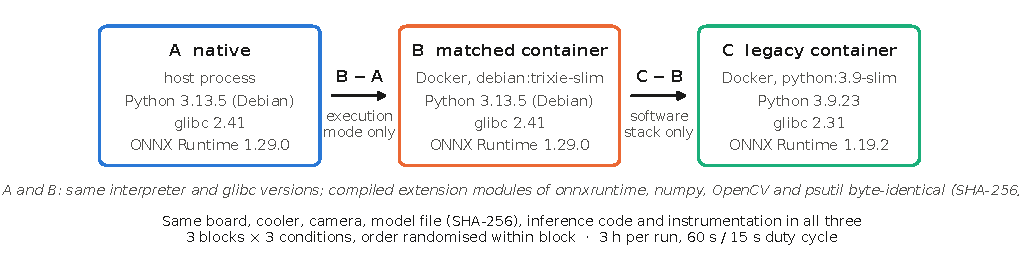
\includegraphics[width=\textwidth]{fig1_design}
\caption{Three-condition design. $B-A$ changes only the execution mode; $C-B$ changes only the software stack inside the image. Versions are those recorded by the environment fingerprints (Table~\ref{tab:stacks}).}
\label{fig:design}
\end{figure*}

% =====================================================================
\section{Related Work}\label{sec:related}

\subsection{Container overhead}
On server hardware, containers have been found to add little CPU overhead relative to native execution, with costs concentrated in I/O and networking paths~\cite{felter2015updated,morabito2015hypervisors}. Studies on ARM single-board computers and IoT devices report a similar picture for CPU-bound work~\cite{morabito2016performance,morabito2017virtualization,ramalho2016virtualization} and have established that Docker-based fog deployments on the Raspberry Pi are feasible~\cite{bellavista2017feasibility}. More recent work compares container engines~\cite{baresi2024qualitative} and contrasts containers with microVMs for edge I/O~\cite{lee2026performance}. Energy has received less attention. Santos et~al.\ measured the energy of workloads run inside and outside Docker on an x86 machine~\cite{santos2018docker}, and Raza et~al.\ compared the performance and energy of container orchestrators on Raspberry Pi gateways~\cite{raza2021empirical}. These studies compare execution environments; none holds the software stack fixed while varying the execution mode for an inference workload. Knoche and Eichelberger used Docker on the Raspberry Pi to make performance experiments replicable, observed a small performance cost and higher variance, and noted that recreating a software environment is hard once particular library versions are no longer available~\cite{knoche2018using}. The present design treats the stack inside the image as a factor in its own right.

\subsection{Inference performance and energy at the edge}
Characterisations of deep neural network inference on commercial edge devices report latency, throughput and power across devices and frameworks~\cite{hadidi2019characterizing,liang2020ai,baller2021deepedgebench}, and benchmark suites standardise the workloads and run rules~\cite{reddi2020mlperf,banbury2021mlperftiny}. Energy measurement on embedded AI devices has its own metrological difficulties~\cite{apicella2026energy}, and Raspberry Pi power has been modelled against utilisation~\cite{kaup2014powerpi}. Long-running inference on CPU-based edge devices interacts with thermal management~\cite{benoitcattin2020impact}. The case for reporting the energy of machine learning, not only its accuracy, is made in~\cite{schwartz2020green,strubell2019energy,henderson2020towards}, and the observation that idle power dominates lightly loaded systems goes back to the argument for energy-proportional computing~\cite{barroso2007case}. Benchmarks usually report energy while the workload is running. A duty-cycled node also spends energy while it waits, and we report both.

\subsection{Dependency staleness and measurement practice}
Developers frequently leave library dependencies outdated~\cite{kula2018developers}, and container images on public registries often carry outdated packages with known vulnerabilities and bugs~\cite{zerouali2019relation,shu2017study}. Deep learning frameworks exhibit performance bugs~\cite{makkouk2022empirical}, and framework versions can change model behaviour~\cite{shahriari2022how}. Staleness is therefore a property of real images, not a contrived condition. On method, small changes to the experimental setup can bias performance results~\cite{mytkowicz2009producing}; statistically rigorous comparison requires repeated independent runs and interval estimates~\cite{georges2007statistically,kalibera2013rigorous,hoefler2015scientific}; and repeated measurements within one run are not independent replicates~\cite{hurlbert1984pseudoreplication}. We follow these practices: the replicate is the three-hour run, and inference is made across runs.

% =====================================================================
\section{Measurement System and Design}\label{sec:method}

\subsection{Node and workload}
The node is a Raspberry Pi~5 (8~GB, four Cortex-A76 cores, 2.4~GHz maximum) with the official Active Cooler, a temperature-controlled fan. It runs Raspberry Pi OS based on Debian~13 (kernel 6.18.39) with the \texttt{ondemand} frequency governor. Power enters through a Waveshare UPS HAT~(E), which supplies the board from a USB Type-C input and holds a four-cell lithium-ion pack. A USB camera delivers 640$\times$480 frames.

The workload is a three-class MobileNetV2 image classifier~\cite{sandler2018mobilenetv2} built for greenhouse crop monitoring and exported to ONNX. The identical model file (SHA-256 recorded for every run) is executed by ONNX Runtime~\cite{onnxruntime} on the CPU execution provider with default session options. Each frame is resized, centre-cropped to 224$\times$224, converted to RGB and normalised; only the inference call is timed, with the wall clock. The application follows the deployed duty cycle: 60~s of continuous capture and inference, then 15~s in which the process sleeps with the camera open. The loop is camera-bound at 15~frame/s, so the number of inferences per cycle is set by the camera, not by inference speed. Each frame appends one record to a CSV log.

\subsection{Conditions}
Table~\ref{tab:stacks} lists the three software stacks.

\emph{A (native)} runs the harness directly on the host in a Python virtual environment on the distribution interpreter.

\emph{B (matched container)} runs the same harness in Docker. Its image definition was generated from the host environment by a script that reads the interpreter version and the installed package versions and emits pins. It starts from \texttt{debian:trixie-slim}, installs the distribution's \texttt{python3} package, and installs the same package versions into a virtual environment. A fingerprinting script records the Python and glibc versions, the ONNX Runtime build string, and the SHA-256 of the compiled extension module of each imported numerical package (ONNX Runtime, NumPy, OpenCV, psutil). The host and B fingerprints are identical in every field. The check does not hash the interpreter binary, the C library or the shared libraries bundled with the wheels, so ``matched'' means the same versions of these and byte-identical extension modules, not a byte-identical file system.

\emph{C (legacy container)} runs the harness in an image built from \texttt{python:3.9-slim-bullseye}, reconstructing the first campaign's image. Its ONNX Runtime is ten minor releases older than the host's and is a different build; NumPy, OpenCV, psutil, Python and glibc also differ. Section~\ref{sec:deviations} describes the reconstruction.

The containers receive the camera and the I\textsuperscript{2}C bus as devices and mount the host time zone. No CPU quota was set (cgroup \texttt{cpu.max} was \texttt{max 100000} in every container run), and all four cores were available to every condition. Apart from the deviations in Section~\ref{sec:deviations}, the model, the inference code, the camera settings and the instrumentation were the same in all three.

\begin{table*}[t]
\centering
\caption{Software stacks as recorded by the environment fingerprints. A and B agree in every recorded field, including the SHA-256 of each compiled extension module. The legacy ONNX Runtime build string records its compiler flags; the host build string records none.}
\label{tab:stacks}
\footnotesize
\begin{tabular}{llll}
\toprule
 & A native & B matched container & C legacy container \\
\midrule
Base & host (Debian 13) & \texttt{debian:trixie-slim} & \texttt{python:3.9-slim-bullseye} (Debian 11)\\
Python & 3.13.5 (Debian package) & 3.13.5 (Debian package) & 3.9.23 (image build) \\
glibc & 2.41 & 2.41 & 2.31 \\
ONNX Runtime & 1.29.0 (build 2e2543fbe9) & 1.29.0 (build 2e2543fbe9) & 1.19.2 (build ffceed9d44)\\
NumPy / OpenCV (headless) & 2.5.2 / 5.0.0.93 & 2.5.2 / 5.0.0.93 & 1.26.4 / 4.10.0.84 \\
psutil / smbus2 & 7.2.2 / 0.6.1 & 7.2.2 / 0.6.1 & 6.1.0 / 0.5.0 \\
\bottomrule
\end{tabular}
\end{table*}

\subsection{Instrumentation}
Three logs are written per run. The per-frame log records inference latency (0.1~ms resolution), system-wide CPU utilisation since the previous frame, memory utilisation, SoC temperature and the latest supply reading. A 1~Hz sampler, running in both phases of the cycle, records the UPS HAT's Type-C bus voltage, current and power; battery voltage, current and charge; SoC temperature and CPU utilisation; the current and capped CPU frequency and the under-voltage alarm; and fan speed and PWM level. The frequency, alarm and fan values are read from sysfs in the same way in all three conditions, so that no condition carries instrumentation load that the others do not. A third log marks cycle transitions. A provenance record captures the kernel, governor, cgroup limits, CPU affinity, library versions and model hash at the start of each run.

The power figure is \emph{node input power}: the power entering the UPS HAT's Type-C input, which covers the board, the fan, the camera and the HAT's own conversion losses. It is not the SoC rail. The HAT reports bus power and bus current in separate registers. Run means of bus current and of power divided by voltage agreed within \PVIDev\% in every run; individual samples scatter more, because the registers update asynchronously. This checks the telemetry's internal consistency, not its absolute accuracy, which the vendor does not specify. Because all conditions are measured with the same instrument and compared as differences within blocks, a constant gain or offset error largely cancels.

The charger remained connected. A run started only once the battery was floating (charge current $\le$50~mA). Over whole runs, the mean battery current was \BatIMeanMin--\BatIMeanMax~mA and never left \BatIMin\ to \BatIMax~mA, so charging diverted at most about \BatWMax~W of bus power on average.

\subsection{Design and protocol}
The design is a randomised complete block design with three blocks and the three conditions in each, the order within each block drawn at random with a fixed seed. A block is one session of three consecutive runs. Each run lasted three hours (144 duty cycles). The first \WarmupS~s of each run were excluded as warm-up, leaving \CyclesAnalysed\ complete cycles per run for analysis. Before each run the orchestrating script waited for the SoC to cool to 50~$^\circ$C or below and for the battery to float, then started the run and checked its completeness and frame count afterwards.

For the whole campaign, all systemd timers were stopped so that no scheduled job could change the host stack or add load mid-run, and no interactive work was done on the node. The graphical desktop session remained running in all nine runs, at under 1\% CPU. The host stack was not modified between the fingerprinting and the last run.

\subsection{Energy accounting}\label{sec:energy}
Let $\bar P_{\mathrm{act}}$ and $\bar P_{\mathrm{slp}}$ be the mean node input power over the active and sleep phases, $T_{\mathrm{act}}$ and $T_{\mathrm{slp}}$ the mean phase durations (\TActS~s and \TSlpS~s), and $f$ the inference rate during the active phase. The energy the node spends per inference over the duty cycle is
\begin{equation}
E_{\mathrm{cyc}} = \frac{\bar P_{\mathrm{act}}T_{\mathrm{act}}+\bar P_{\mathrm{slp}}T_{\mathrm{slp}}}{f\,T_{\mathrm{act}}}. \label{eq:cyc}
\end{equation}
The sleep phase does not reach its floor immediately. The \texttt{ondemand} governor held the maximum frequency for about 5~s after each active phase ended, and the node drew \HoldWlo--\HoldWhi~W more during those seconds than later in the sleep phase. We therefore define the settled floor $P_{\mathrm{floor}}$ as the mean power over sleep-phase samples taken at least \SettleS~s after the phase began, and split $E_{\mathrm{cyc}}$ into a baseline and a workload increment:
\begin{align}
E_{\mathrm{base}} &= \frac{P_{\mathrm{floor}}\,(T_{\mathrm{act}}+T_{\mathrm{slp}})}{f\,T_{\mathrm{act}}}, \label{eq:base}\\
E_{\mathrm{inc}} &= E_{\mathrm{cyc}} - E_{\mathrm{base}}. \label{eq:inc}
\end{align}
$E_{\mathrm{base}}$ is what the node would spend per inference if it drew only its floor for the whole cycle; $E_{\mathrm{inc}}$ is the energy above that floor, including the governor's hold after each active phase. The floor is not a hardware idle state. The process stays resident with the camera open and the desktop running, so $P_{\mathrm{floor}}$ is the node's floor under this software configuration, not the hardware's minimum.

\subsection{Statistical analysis}
The unit of replication is the run. For each quantity, a run-level value is computed over the post-warm-up period. An effect such as $B-A$ is estimated as the mean of the three within-block differences, with a 95\% confidence interval from the $t$ distribution with two degrees of freedom. With three blocks the intervals are wide, and we report them rather than $p$-values, together with the sign of the difference in each block. Percentages are relative to the reference condition of each contrast (A for $B-A$, B for $C-B$). Mean latency and energy per inference above the floor and over the cycle are the quantities of primary interest; the others are reported for completeness, and their intervals are not adjusted for multiplicity.

\subsection{Deviations from protocol}\label{sec:deviations}
Four events are reported so that readers can judge them.

\emph{Camera frame rate.} The camera's default exposure mode lowers its frame rate in low light. The first two runs (\texttt{legacy\_1} and \texttt{matched\_1}) ran in a dark room and held 15.0~frame/s in every hour. In the next run, the original \texttt{native\_1}, the operator saw the frame rate rise when the room lights came on; the run was stopped and its partial logs were not kept. From the following run (\texttt{legacy\_2}) onward, dynamic frame rate was disabled on the host before every run, 15~frame/s was requested explicitly, and the camera controls were saved with each run.

\emph{Harness update and image rebuild.} To request the frame rate, the harness was updated after the second run; the change also added a measured-rate line to the run summary and did not touch the preprocessing, the timed inference call or the per-frame logging (the earlier version of the harness was not retained). Both images were rebuilt to include the new harness. The harness is copied in the images' final layer, after the layers that install the software stack, so unless the build cache is bypassed a rebuild reuses the stack layers. The binary fingerprints were taken before the first run and were not repeated after the rebuild, but the per-run provenance records show the same interpreter, C library, ONNX Runtime, NumPy and OpenCV versions in every run of each condition. Within block~1, B ran with the camera unpinned at \FPSEarlyMax~frame/s and A with the camera pinned.

\emph{Block~1 timing.} The replacement \texttt{native\_1} ran in the evening of the same day (20:19--23:19 local time), after block~2, and was not contiguous with the other block~1 runs. Section~\ref{sec:sens} repeats the analysis without block~1.

\emph{Legacy image reconstruction.} The first campaign's image no longer existed, so condition~C was rebuilt from its definition. That definition did not pin package versions. The base image fixes Python~3.9, and ONNX Runtime~1.19.2 is the only release that fits it, being the last with a wheel for that interpreter on 64-bit ARM. The other packages were pinned to the versions in Table~\ref{tab:stacks}; it cannot be shown that the original build resolved the same versions. One system package in the definition (\texttt{libglib2.0-0}) is no longer available from the base distribution's archive and was omitted; the headless OpenCV build does not require it. Condition~C therefore reproduces the first campaign's Python minor version and runtime, but it is not a copy of that image.

Run start times, per-run tables and fingerprints are given in the supplemental material.

% =====================================================================
\section{Results}\label{sec:results}

\subsection{Run integrity}
All nine runs completed, each with \TotFramesMin--\TotFramesMax\ inferences (\FramesAll\ in total). The inference rate was \FPSPinnedMin--\FPSPinnedMax~frame/s in the seven runs with the camera pinned and \FPSEarlyMin~frame/s in the two early runs. No 1~Hz sample showed a CPU frequency cap below 2400~MHz (\CapSamples\ samples) or an under-voltage alarm (\UVSamples\ samples), and the mean active-phase frequency was at least \MHzMin~MHz in every run. The highest SoC temperature recorded in any run was \TMaxAll~$^\circ$C. Every run used the same model file. Table~\ref{tab:results} gives the condition means and both contrasts; Fig.~\ref{fig:decomp} shows the contrasts as percentages.

\begin{table*}[t]
\centering
\caption{Condition means ($\pm$ SD over three runs) and within-block effects with 95\% confidence intervals ($t$, 2 d.f.). $^{\dagger}$: interval includes zero. Signs: direction of the difference in blocks 1, 2 and 3. CPU utilisation is system-wide, sampled per frame in the active phase. The settled floor is the sleep-phase power after the governor has stepped down; energy per inference above the floor and over the whole duty cycle are defined in Section~\ref{sec:energy}.}
\label{tab:results}
\setlength{\tabcolsep}{3.5pt}
\scriptsize
\begin{tabular}{lccc ccc ccc}
\toprule
 & \multicolumn{3}{c}{Condition mean $\pm$ SD} & \multicolumn{3}{c}{$B-A$ (execution mode)} & \multicolumn{3}{c}{$C-B$ (software stack)}\\
\cmidrule(lr){2-4}\cmidrule(lr){5-7}\cmidrule(lr){8-10}
Quantity & A native & B matched & C legacy & effect & 95\% CI & signs & effect & 95\% CI & signs\\
\midrule
Inference rate (frame/s) & 14.90 $\pm$ 0.02 & 14.95 $\pm$ 0.09 & 14.94 $\pm$ 0.09 & +0.05$^{\dagger}$ & [\textminus 0.14, 0.24] & +$-$+ & \textminus 0.01$^{\dagger}$ & [\textminus 0.03, 0.01] & $-$$-$$-$\\
Latency, mean (ms) & 19.37 $\pm$ 0.14 & 20.68 $\pm$ 0.41 & 29.26 $\pm$ 0.82 & +1.30 & [0.52, 2.08] & +++ & +8.58 & [5.81, 11.35] & +++\\
Latency, median (ms) & 20.20 $\pm$ 0.17 & 20.83 $\pm$ 1.44 & 27.10 $\pm$ 2.31 & +0.63$^{\dagger}$ & [\textminus 2.76, 4.02] & +0$-$ & +6.27$^{\dagger}$ & [\textminus 2.30, 14.84] & +++\\
Latency, p95 (ms) & 26.00 $\pm$ 0.61 & 26.20 $\pm$ 1.04 & 41.57 $\pm$ 1.96 & +0.20$^{\dagger}$ & [\textminus 3.30, 3.70] & $-$++ & +15.37 & [8.10, 22.64] & +++\\
Latency, p99 (ms) & 28.90 $\pm$ 0.80 & 31.45 $\pm$ 1.51 & 43.83 $\pm$ 0.15 & +2.55$^{\dagger}$ & [\textminus 1.79, 6.90] & +++ & +12.38 & [8.98, 15.78] & +++\\
CPU utilisation, system (\%) & 56.1 $\pm$ 0.2 & 57.3 $\pm$ 0.7 & 48.6 $\pm$ 0.4 & +1.3$^{\dagger}$ & [\textminus 0.1, 2.6] & +++ & \textminus 8.8 & [\textminus 10.8, \textminus 6.8] & $-$$-$$-$\\
CPU time per inference (ms) & 150.6 $\pm$ 0.4 & 153.4 $\pm$ 0.9 & 130.0 $\pm$ 1.4 & +2.8 & [0.9, 4.8] & +++ & \textminus 23.4 & [\textminus 28.4, \textminus 18.3] & $-$$-$$-$\\
Power, active phase (W) & 10.46 $\pm$ 0.08 & 10.51 $\pm$ 0.03 & 9.81 $\pm$ 0.19 & +0.06$^{\dagger}$ & [\textminus 0.08, 0.19] & +++ & \textminus 0.70 & [\textminus 1.20, \textminus 0.20] & $-$$-$$-$\\
Power, sleep phase (W) & 6.97 $\pm$ 0.05 & 6.95 $\pm$ 0.02 & 6.81 $\pm$ 0.20 & \textminus 0.02$^{\dagger}$ & [\textminus 0.14, 0.11] & $-$$-$+ & \textminus 0.14$^{\dagger}$ & [\textminus 0.67, 0.39] & $-$+$-$\\
Power, settled floor (W) & 6.61 $\pm$ 0.06 & 6.60 $\pm$ 0.05 & 6.54 $\pm$ 0.18 & \textminus 0.02$^{\dagger}$ & [\textminus 0.11, 0.08] & $-$$-$+ & \textminus 0.06$^{\dagger}$ & [\textminus 0.53, 0.41] & $-$+$-$\\
Energy/inference above floor (mJ) & 263.9 $\pm$ 1.1 & 267.9 $\pm$ 3.1 & 224.2 $\pm$ 9.5 & +4.0$^{\dagger}$ & [\textminus 6.3, 14.4] & $-$++ & \textminus 43.8 & [\textminus 60.0, \textminus 27.5] & $-$$-$$-$\\
Energy/inference, cycle (mJ) & 818.8 $\pm$ 5.4 & 819.5 $\pm$ 2.4 & 770.9 $\pm$ 17.7 & +0.7$^{\dagger}$ & [\textminus 18.6, 20.0] & $-$++ & \textminus 48.6 & [\textminus 89.8, \textminus 7.5] & $-$$-$$-$\\
Cyclic peak temperature ($^\circ$C) & 64.9 $\pm$ 1.5 & 64.3 $\pm$ 0.3 & 61.6 $\pm$ 1.9 & \textminus 0.6$^{\dagger}$ & [\textminus 3.6, 2.4] & $-$+$-$ & \textminus 2.7$^{\dagger}$ & [\textminus 7.9, 2.5] & $-$$-$$-$\\
Fan speed, active phase (rpm) & 5336 $\pm$ 192 & 5234 $\pm$ 69 & 4521 $\pm$ 712 & \textminus 101$^{\dagger}$ & [\textminus 454, 252] & $-$+$-$ & \textminus 713$^{\dagger}$ & [\textminus 2567, 1140] & $-$+$-$\\
\bottomrule
\end{tabular}
\end{table*}


\subsection{Latency}
Mean inference latency was \LatMeanA, \LatMeanB\ and \LatMeanC~ms in A, B and C. The containerisation effect $B-A$ was \LatMeanBAabs~ms (\LatMeanBApctabs\%, 95\% CI \LatMeanBAlo\ to \LatMeanBAhi~ms) and positive in all three blocks. The stack effect $C-B$ was \LatMeanCBabs~ms (\LatMeanCBpctabs\%, CI \LatMeanCBlo\ to \LatMeanCBhi~ms), also positive in every block. Of the total difference between the legacy container and native execution, $C-A=\LatMeanCAabs$~ms, the execution mode accounts for \ShareContainer\% and the stack for \ShareStack\%.

The distributions (Fig.~\ref{fig:latency}) show that the two effects differ in kind. A and B share the same fast mode: their per-run first percentiles were \PoneAlo--\PoneAhi\ and \PoneBlo--\PoneBhi~ms, and their fastest inferences \LatMinA\ and \LatMinB~ms. What differs is how often an inference falls in that mode: \FastAlo--\FastAhi\% of inferences took under \FastMs~ms in the native runs against \FastBlo--\FastBhi\% in the matched-container runs. Containerisation did not slow the fastest inferences; it made fast inferences less frequent. The legacy stack shifted the whole distribution: its first percentile was \PoneClo--\PoneChi~ms and its fastest inference \LatMinC~ms. At the tail, $B-A$ was not resolved (p95 \LatPninetyfiveBA~ms, CI \LatPninetyfiveBAlo\ to \LatPninetyfiveBAhi; p99 \LatPninetynineBA~ms, CI \LatPninetynineBAlo\ to \LatPninetynineBAhi), whereas $C-B$ was \LatPninetyfiveCBabs~ms at p95 (\LatPninetyfiveCBpctabs\%) and \LatPninetynineCBabs~ms at p99.

\begin{figure}[t]
\centering
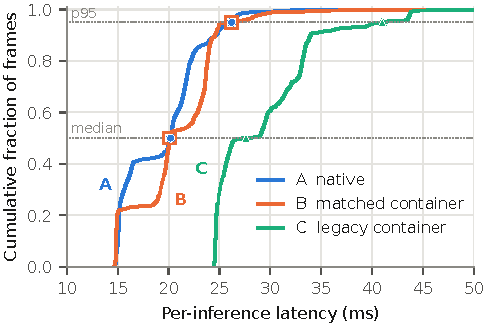
\includegraphics[width=\columnwidth]{fig2_latency}
\caption{Empirical distribution of per-inference latency, pooled over the three runs of each condition after warm-up. Markers show the pooled median and 95th percentile; B's markers are drawn hollow because they coincide with A's.}
\label{fig:latency}
\end{figure}

\begin{figure*}[t]
\centering
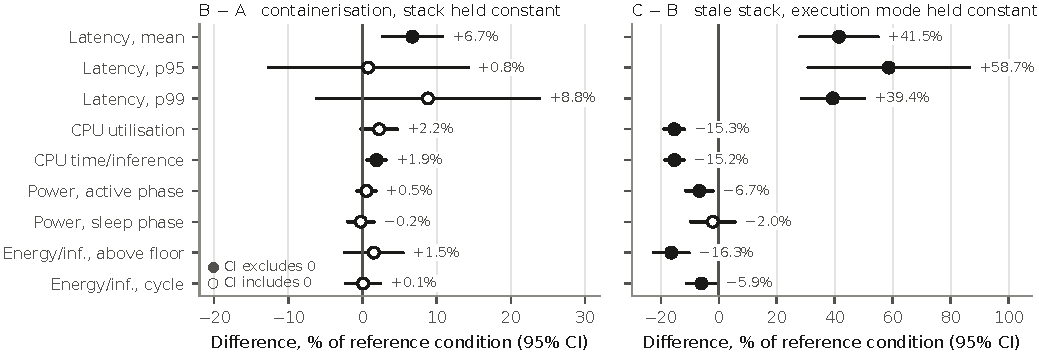
\includegraphics[width=\textwidth]{fig3_decomposition}
\caption{The two contrasts as percentages of the reference condition, with 95\% confidence intervals from three within-block differences ($t$, 2 d.f.). Filled markers: interval excludes zero. CPU time per inference is system-wide CPU utilisation $\times$ four cores / inference rate.}
\label{fig:decomp}
\end{figure*}

\subsection{Processor load, power and energy}
Containerisation raised processor load slightly. System-wide CPU utilisation was \CPUBAabs\ percentage points higher in B than in A, positive in all three blocks but with an interval that includes zero (\CPUBAlo\ to \CPUBAhi). Expressed as CPU time per inference (utilisation $\times$ four cores / inference rate), which removes the small frame-rate differences between runs, the effect was \CPUmsBAabs~ms (\CPUmsBApctabs\%, CI \CPUmsBAlo\ to \CPUmsBAhi~ms). Power did not change detectably: $B-A$ was \PActBA~W in the active phase (CI \PActBAlo\ to \PActBAhi) and \PSlpBA~W in the sleep phase. Energy per inference above the floor was \EIncBA~mJ (\EIncBApct\%, CI \EIncBApctlo\% to \EIncBApcthi\%), and over the cycle \ECycBA~mJ (\ECycBApct\%, CI \ECycBApctlo\% to \ECycBApcthi\%). Effects on cycle energy of more than a few percent are therefore excluded; smaller ones are not.

The stack effect runs against the latency result. With the older stack, CPU utilisation was \CPUCBabs\ percentage points lower (\CPUCBpct\%, CI \CPUCBlo\ to \CPUCBhi) and CPU time per inference \CPUmsCBabs~ms lower (\CPUmsCBpct\%). Active-phase power was \PActCBabs~W lower (\PActCBpct\%, CI \PActCBlo\ to \PActCBhi~W), while the settled floor did not differ detectably (\PFloorCB~W). Energy per inference above the floor, Eq.~\eqref{eq:inc}, was \EIncCBabs~mJ lower (\EIncCBpct\%, CI \EIncCBlo\ to \EIncCBhi~mJ, negative in every block), and energy per inference over the cycle, Eq.~\eqref{eq:cyc}, was \ECycCBabs~mJ lower (\ECycCBpct\%, CI \ECycCBlo\ to \ECycCBhi~mJ). Relative to the legacy stack, then, the current stack takes \StackTimeSavedPct\% less time per inference call and spends \StackIncExtraPct\% more energy above the floor on each inference. It also uses about \CPUmsCBabsInt~ms more CPU time per inference while finishing the timed call about \LatMeanCBabsOne~ms sooner, which is consistent with more cores being busy during each call. This CPU time covers the whole process and the system, not only the inference call.

Part of the power difference is the fan. The fan draws from the same supply, and in blocks 1 and 3 the legacy run's fan was slower than the matched run's, by \FanCBblkOneabs\ and \FanCBblkThreeabs~rpm. In block~2, however, where the legacy fan ran \FanCBblkTwoabs~rpm faster, active power was still \PActCBblkTwoabs~W lower, so the power difference is not explained by the fan alone.

Fig.~\ref{fig:energy} splits energy per inference over the cycle into the baseline, Eq.~\eqref{eq:base}, and the increment. The baseline was \EBaseA, \EBaseB\ and \EBaseC~mJ in A, B and C, or \EBaseShareA, \EBaseShareB\ and \EBaseShareC\% of the total. The resolved part of the stack effect lies in the increment, which carries \IncShareOfStackEnergy\% of the $C-B$ difference in cycle energy.

\begin{figure}[t]
\centering
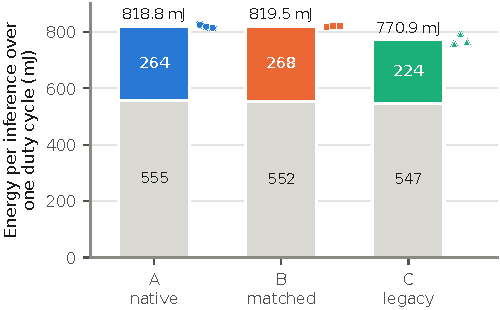
\includegraphics[width=\columnwidth]{fig4_energy}
\caption{Energy per inference over one 60~s/15~s duty cycle, Eq.~\eqref{eq:cyc}. Grey: baseline at the settled sleep-phase floor, Eq.~\eqref{eq:base}; colour: increment above the floor, Eq.~\eqref{eq:inc}; markers: individual runs. Totals are condition means.}
\label{fig:energy}
\end{figure}

\subsection{Temperature and fan}
Mean cyclic peak SoC temperature was \TPeakA, \TPeakB\ and \TPeakC~$^\circ$C (Fig.~\ref{fig:thermal}). Neither contrast was resolved. $B-A$ was \TPeakBA~$^\circ$C (CI \TPeakBAlo\ to \TPeakBAhi). $C-B$ was \TPeakCB~$^\circ$C (CI \TPeakCBlo\ to \TPeakCBhi); it was negative in all three blocks but ranged from \TPeakCBblkmin\ to \TPeakCBblkmax~$^\circ$C. Active-phase fan speed moved the same way on average ($C-B$ \FanCB~rpm, CI \FanCBlo\ to \FanCBhi). The fan controller regulates temperature, so part of any difference in heat output appears as fan speed rather than as temperature, and the two readings must be read together. In block~2 the legacy run's fan ran slightly faster than the matched run's, and its peak temperature was within \TPeakCBblkTwoabs~$^\circ$C of it.

\begin{figure}[t]
\centering
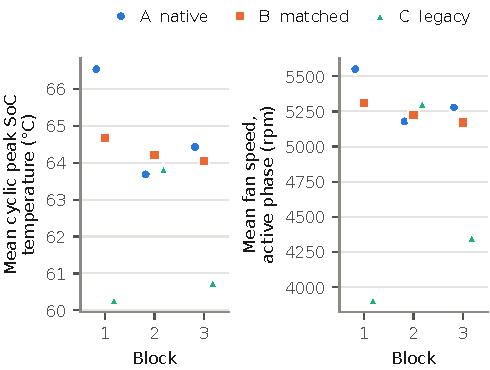
\includegraphics[width=\columnwidth]{fig5_thermal}
\caption{Mean cyclic peak SoC temperature (left) and mean active-phase fan speed (right) for each run, by block. The Active Cooler's fan is temperature-controlled, so the two panels are coupled.}
\label{fig:thermal}
\end{figure}

\subsection{Sensitivity and relation to the first campaign}\label{sec:sens}
Excluding block~1, whose native run was repeated later and whose matched run had the camera unpinned, leaves two blocks. The point estimates change little: $B-A$ latency \LatMeanBAsens~ms and $C-B$ latency \LatMeanCBsens~ms (\LatMeanBA\ and \LatMeanCB~ms with all blocks); $C-B$ energy per inference above the floor \EIncCBsens~mJ (\EIncCB). With two blocks the intervals use $t_{0.975,1}=12.7$ and widen sharply: the $B-A$ latency interval then includes zero (\LatMeanBAsenslo\ to \LatMeanBAsenshi~ms), while the $C-B$ intervals for latency (\LatMeanCBsenslo\ to \LatMeanCBsenshi~ms) and energy above the floor (\EIncCBsenslo\ to \EIncCBsenshi~mJ) still exclude it. One estimate sharpens. In blocks 2 and 3, $B-A$ energy above the floor was \EIncBAsens~mJ (\EIncBAsenspct\%), and its two-block interval (\EIncBAsenslo\ to \EIncBAsenshi~mJ) excludes zero. Block~1 is the only block with a negative $B-A$ difference in this quantity (\EIncBAblkOne~mJ), and it is the block in which B ran with the camera unpinned at a slightly higher frame rate. Containerisation therefore probably costs a small amount of workload energy, of the order of 2\% of the energy above the floor, or \ECycBAsenspct\% of the energy per inference over the cycle.

The first campaign~\cite{lin2026dataset} used an older harness with a lower frame rate, two runs per condition and no idle measurement, so its values are not pooled with these. Its contrast corresponds to $C-A$ here, and every sign reproduces: mean latency +\LatMeanCApctabs\% (first campaign +\FirstLatPct\%), CPU utilisation \CPUCAabs\ percentage points lower (\FirstCPUpp), active power \PActCAabs~W lower (\FirstPW~W) and cyclic peak temperature \TPeakCAabs~$^\circ$C lower (\FirstPeak~$^\circ$C). The difference is in interpretation: the present design shows that most of that contrast comes from the stack in the image, not from running in a container.

% =====================================================================
\section{Discussion}\label{sec:discussion}

\subsection{What a container-versus-native figure measures}
Unless the stacks are verified equal, a comparison between a containerised deployment and native execution measures two things. On this node, the execution-mode component is small: \LatMeanBAabs~ms of mean latency, \CPUmsBApctabs\% of CPU time per inference, no detectable change in power or temperature, and probably about 2\% of the energy above the floor. The software-stack component is about \StackToContainerRatio\ times larger in latency and determines the energy result. A study that reports the joint figure as container overhead will overstate it; one that happened to package a newer stack than the host's could understate it or reverse its sign. The practical requirement is cheap. Record the interpreter, the C library, and the versions and hashes of the numerical binaries in each condition, and either match them or report the mismatch as a factor. The fingerprinting and Dockerfile-generation scripts released with this paper do this in seconds; hashing the interpreter, the C library and the bundled shared libraries as well would make the check stricter.

The containerisation effect that remains is informative. It did not raise the latency floor, which is inconsistent with a constant cost added to every call. Instead, it lowered the frequency of the fast mode. A change in how often the fast path is taken is more consistent with an interaction with scheduling, core placement or cache state than with added instructions on every call. The present measurements cannot identify it. Hardware performance counters and scheduler tracing, which we did not collect so as to keep the instrumentation light and identical in all conditions, are the tools for that question.

\subsection{A faster stack is not a cheaper one}
The current stack finished each inference call in \StackTimeSavedPct\% less time than the older one and spent more energy doing so. The loop is camera-bound, so finishing sooner does not produce more inferences; it only lengthens the wait before the next frame. Whether a faster inference saves energy then depends on how much power is drawn while it runs and whether the cores return to a low-power state between frames. Here the current stack drew more power during the active phase than its shorter calls could repay, consistent with its higher CPU time per inference. Updating the software stack to reduce latency can therefore increase the energy of a rate-limited edge node. Conversely, a stale image can look more energy-efficient than a current one for reasons that have nothing to do with containerisation. Energy comparisons across deployment configurations should state the runtime and library versions and, for rate-limited loops, report energy per inference and not latency alone. The $C-B$ contrast changes the whole stack, so the present data do not say which component is responsible. Runtime session options, such as the number of intra-operator threads and whether idle worker threads spin, are candidates that a follow-up study can vary directly, alongside the library versions.

\subsection{The idle floor dominates}
On this node, \EBaseShareLo--\EBaseShareHi\% of the energy per inference over the duty cycle is accounted for by the settled sleep-phase floor drawn over the whole cycle, and that share hardly depended on the condition. The largest effect on energy per inference over the cycle, the stack effect, was \ECycCBpctabs\%. For sustainability, the software stack matters, but the platform's floor matters more: the desktop session, the open camera, the fan and the conversion losses of the supply board contribute to it. Reducing that floor, for example by running headless, releasing the camera during the wait, or entering a deeper idle state, is a larger lever than any choice among the three conditions studied here, although we did not measure these alternatives. The governor's hold at maximum frequency after each active phase cost about \HoldmJ~mJ per inference, small by comparison. This is the energy-proportionality argument~\cite{barroso2007case} at the scale of a single edge node. It also means that energy figures reported without the idle phase describe only the smaller part of what a duty-cycled node consumes.

\subsection{Thermal effects under active cooling}
With a temperature-controlled fan, a difference in heat output shows up partly as a temperature difference and partly as a fan-speed difference. The older stack's lower power was accompanied by lower cyclic peaks and a slower fan in blocks 1 and 3, and by a slightly faster fan with almost no temperature difference in block~2. The within-block order also matters here. In blocks 1 and 3 the legacy runs fell in the pre-dawn hours, which are usually the coolest, whereas in block~2 the legacy run was at midday. Ambient temperature was not logged, so an ambient contribution to the thermal and fan differences in blocks 1 and 3 cannot be excluded. For thermal comparisons on actively cooled boards, temperature alone can hide a real difference in heat, and the fan's state and the ambient temperature should be logged alongside it.

\subsection{Limitations}
The results come from one board, one model, one pair of software stacks and one duty cycle, and they should be read as a controlled case study, not as general constants. Three blocks give wide intervals: the $B-A$ energy and thermal contrasts are consistent with zero over all blocks, and the small $B-A$ energy effect suggested by blocks 2 and 3 rests on two blocks. The $C-B$ contrast bundles the whole stack; the inference call is the timed region, which points towards the runtime, but Python, NumPy, OpenCV and glibc also changed and were not varied separately. ONNX Runtime thread counts and spinning behaviour were left at their defaults and not recorded at run time. Power is node input power sampled at 1~Hz from a module with unspecified absolute accuracy; differences between conditions are more trustworthy than absolute values, and the fan's share of the power difference was not measured separately. Ambient temperature was not logged; the blocks remove variation between sessions, not within them. The floor is not a hardware idle state, and the governor was \texttt{ondemand} throughout; a different governor or a deeper idle state would change the baseline and possibly the stack effect. Block~1 was not contiguous and ran B with the camera unpinned. The images were rebuilt once during the campaign, and the legacy image was reconstructed from its definition rather than reused.

% =====================================================================
\section{Conclusion}\label{sec:conclusion}
We separated the cost of running an edge inference workload in a container from the cost of the software stack that the container carried. With the interpreter, C library and numerical extension modules held the same, containerisation added \LatMeanBAabs~ms (\LatMeanBApctabs\%) to mean inference latency and \CPUmsBApctabs\% to CPU time per inference, no resolvable change in power or temperature, and probably about 2\% to the energy above the idle floor. The older stack found in a real image accounted for \ShareStack\% of the latency difference, and it was the less energy-hungry configuration: \EIncCBpctabs\% less energy per inference above the idle floor and \ECycCBpctabs\% less over the duty cycle, with lower active power in every block. The idle floor made up \EBaseShareLo--\EBaseShareHi\% of the energy per inference. Container-versus-native comparisons at the edge should therefore verify and report the software stack in each condition, and energy studies of duty-cycled nodes should measure the idle phase. Future work will use hardware performance counters and scheduler tracing to explain the change in the fast-mode frequency under containerisation, and will vary runtime threading options and library versions separately to locate the energy difference between the stacks.

% =====================================================================
\section*{Data and Code Availability}
The per-frame, 1~Hz and cycle-event logs of all nine runs, with their provenance records, camera settings, environment fingerprints and orchestration log, are deposited at Zenodo~\cite{lin2026dataset} together with the first campaign's telemetry. The run kit (harness, orchestrator, image definitions and fingerprinting script) and the analysis and figure scripts, which regenerate every number, table and figure in this paper from the raw logs, are in the \texttt{three\_condition} directory of \url{https://github.com/xiaolin200206/edge-container-deployment-measurement} (release \texttt{v2.0-tsusc}).

\section*{Acknowledgment}
The author used Claude (Anthropic), a generative AI system, throughout this work: to help design the three-condition protocol; to write the measurement harness, orchestration, fingerprinting, analysis and figure scripts; to draft and edit the text of all sections; and to check reference metadata. The author built and operated the hardware, ran all measurements, reviewed all code, text and results, and takes responsibility for the entire content. All numbers in the paper are generated by the released scripts from the raw logs.

\bibliographystyle{IEEEtran}
\bibliography{refs}

\end{document}
